\section{问题重述}
\subsection{研究背景与任务}
\Placeholder{简述研究对象、应用场景和决策需求，提炼题目给定的数据与约束，避免大段照抄赛题。}

\subsection{待解决的问题}
\Placeholder{逐项写清每个问题的输入、所求量、约束与输出形式；按赛题实际设问数量增删。}

\section{问题分析}
\Placeholder{结合图~\ref{fig:route}，说明主要难点、问题之间的依赖关系，以及所选模型的适用性和方法取舍。}
\begin{figure}[htbp]
  \centering
  \FigurePlaceholder{总体建模流程图}
  \caption{\Placeholder{总体建模流程与问题关系}}
  \label{fig:route}
\end{figure}
\FloatBarrier

\section{模型假设}
\begin{enumerate}[label=假设\arabic*：,labelwidth=4em,labelsep=0.5em,leftmargin=4.5em,labelindent=0pt,align=left]
  \item \Placeholder{写明假设内容、题目或数据依据及可能影响的结论范围。}
  \item \Placeholder{补充必要假设，并在后文检验影响结论的关键假设。}
\end{enumerate}

\section{符号说明}
\begin{table}[htbp]
  \centering
  \caption{主要符号及其含义}
  \label{tab:symbols}
  \begin{tabularx}{\linewidth}{L{22mm} Y L{36mm}}
    \toprule
    符号 & 含义 & 单位或范围 \\
    \midrule
    \Placeholder{符号} & \Placeholder{变量或参数定义} & \Placeholder{单位} \\
    \Placeholder{符号} & \Placeholder{变量或参数定义} & \Placeholder{取值范围} \\
    \Placeholder{符号} & \Placeholder{变量或参数定义} & \Placeholder{单位} \\
    \bottomrule
  \end{tabularx}
\end{table}
\FloatBarrier

\section{数据处理}
\subsection{数据来源与质量检查}
\Placeholder{列出附件、字段、样本数量、统计口径及单位。补充数据须注明真实来源和获取日期，说明缺失、异常、重复与测量误差情况。}

\subsection{预处理与特征构造}
\Placeholder{说明缺失值和异常值处理、量纲统一与特征构造。预测任务应交代训练、验证和测试划分，避免未来信息泄漏。}

\section{问题一的模型建立与求解}
\subsection{变量定义与模型建立}
\Placeholder{给出变量、参数、目标、约束及推导或真实引用依据。式~\eqref{eq:model} 仅演示公式格式，须替换为实际模型；引用样式见文献\cite{book-placeholder}，书籍还须在引用处注明页码。}
\begin{equation}
  y=f(\boldsymbol{x};\boldsymbol{\theta})
  \label{eq:model}
\end{equation}
\Placeholder{解释式中各量的含义、单位、范围及边界条件，并与符号表保持一致。}

\subsection{求解算法与实现}
\Placeholder{说明算法步骤、初始化、参数、停止条件、求解器状态和运行环境。随机算法记录种子，按需要报告计算时间。}

\subsection{结果展示与解释}
\begin{table}[htbp]
  \centering
  \caption{\Placeholder{问题一的核心结果}}
  \label{tab:results}
  \begin{tabularx}{\linewidth}{Y Y Y Y}
    \toprule
    对象或方案 & 评价量及单位 & 结果 & 含义 \\
    \midrule
    \Placeholder{对象} & \Placeholder{指标与单位} & \Placeholder{待计算} & \Placeholder{解释} \\
    \Placeholder{对象} & \Placeholder{指标与单位} & \Placeholder{待计算} & \Placeholder{解释} \\
    \bottomrule
  \end{tabularx}
\end{table}
\FloatBarrier
\Placeholder{根据表~\ref{tab:results} 回答问题一的具体设问，解释数量级、约束满足情况及实际意义，保证图表与文字中的数值一致。}

% ============================================================
% 问题二：异构无人机多点多架次运输调度
% ============================================================

% ---------- 问题二最终结果宏 ----------
% 若最终正式运行 q2_solver.py 后结果发生变化，只需修改此处
\newcommand{\QTwoIter}{800}
\newcommand{\QTwoSeed}{20260924}

\newcommand{\QTwoInitTrips}{25}
\newcommand{\QTwoInitMakespan}{13017.522}
\newcommand{\QTwoInitEnergy}{82.8946}
\newcommand{\QTwoInitLate}{139.3771}

\newcommand{\QTwoTrips}{19}
\newcommand{\QTwoMakespan}{9590.134}
\newcommand{\QTwoMakespanHour}{2.664}
\newcommand{\QTwoEnergy}{64.9654}
\newcommand{\QTwoLate}{6.0770}
\newcommand{\QTwoHardViolation}{0}
\newcommand{\QTwoMinSOC}{20.74\%}
\newcommand{\QTwoSoftLateNum}{3}

\newcommand{\QTwoLateImprove}{95.64\%}
\newcommand{\QTwoMakespanImprove}{26.33\%}
\newcommand{\QTwoEnergyImprove}{21.63\%}
\newcommand{\QTwoTripsImprove}{24.00\%}

\section{问题二：异构无人机多点多架次运输调度}
\label{sec:q2}

\subsection{问题分析与总体思路}

问题一仅考虑单服务区直接往返运输，而问题二进一步允许单个运输架次连续访问多个服务区，
同时引入了实体运输无人机、共享电池、充电周转以及不同类别物资的配送时限。
因此，问题二不再是单纯的货箱组批问题，而是一个同时包含
\textbf{货箱分配、服务区访问顺序、运输机型选择、实体无人机分配、共享电池分配和架次开始时刻}
的异构多架次运输调度问题。

若直接将上述决策变量同时编码，一方面搜索空间随货箱数和架次数迅速膨胀，
另一方面还会产生大量违反载质量、体积、能源及时限约束的不可行解。
为此，本文将原问题划分为``路线优化''与``资源调度''两个层次：
上层只确定货箱所属架次以及架次内部服务区访问顺序，
下层通过资源调度解码器自动完成机型、实体无人机、共享电池和开始时刻的配置。
其基本求解链路可表示为
\[
\boxed{
	\text{航段预计算}
	\rightarrow
	\text{单架次评价}
	\rightarrow
	\text{初始路线构造}
	\rightarrow
	\text{ALNS 路线优化}
	\rightarrow
	\text{资源调度解码}
	\rightarrow
	\text{方案可行性检验}
}.
\]

该分层方式将原本高维的联合组合优化问题转化为以
``货箱组批+访问顺序''为核心搜索变量的问题，
而机型与能源资源配置均由确定性的调度解码器生成，
从而显著降低搜索难度。

\subsection{多点运输架次评价模型}

\subsubsection{路线对象与货箱组批}

设全部不可拆货箱集合为
\[
\mathcal{B}=\{1,2,\ldots,N_B\},
\]
本题中 $N_B=80$。
一个运输架次 $r$ 的访问服务区序列表示为
\[
\mathcal{R}_r=
\left[
(i_{r1},\mathcal{B}_{r1}),
(i_{r2},\mathcal{B}_{r2}),
\ldots,
(i_{rK_r},\mathcal{B}_{rK_r})
\right],
\]
其中 $i_{rh}$ 表示架次 $r$ 第 $h$ 个访问的服务区，
$\mathcal{B}_{rh}$ 表示在该服务区交付的货箱集合。
完整飞行路线为
\[
O01\rightarrow i_{r1}\rightarrow i_{r2}
\rightarrow\cdots\rightarrow i_{rK_r}\rightarrow O01.
\]

同一服务区在同一架次内最多访问一次，但允许其货箱分由不同架次配送。
对任意货箱 $b$，要求其恰好被安排一次，即
\begin{equation}
	\sum_{r}x_{br}=1,
	\qquad b\in\mathcal{B},
	\label{eq:q2-box-once}
\end{equation}
其中 $x_{br}=1$ 表示货箱 $b$ 被分配至架次 $r$。

设货箱 $b$ 的质量和体积分别为 $w_b$ 与 $v_b$，
则架次 $r$ 的初始总载质量与总体积为
\begin{equation}
	W_r=\sum_{h=1}^{K_r}\sum_{b\in\mathcal{B}_{rh}}w_b,
	\qquad
	V_r=\sum_{h=1}^{K_r}\sum_{b\in\mathcal{B}_{rh}}v_b.
	\label{eq:q2-capacity-total}
\end{equation}
若架次采用机型 $m$，其最大载质量和最大装载体积分别为
$W_m^{\max}$ 与 $V_m^{\max}$，则必须满足
\begin{equation}
	W_r\le W_m^{\max},
	\qquad
	V_r\le V_m^{\max}.
	\label{eq:q2-capacity}
\end{equation}

由于运输过程中只发生卸货而不再次装货，最大载荷必然出现在从 O01 起飞时。
同时，为准确计算载荷相关能耗，本文按访问顺序更新各航段剩余载荷。
架次在驶向第 $h$ 个服务区时的有效载荷为
\begin{equation}
	q_{rh}
	=
	\sum_{\ell=h}^{K_r}
	\sum_{b\in\mathcal{B}_{r\ell}}w_b,
	\qquad
	h=1,\ldots,K_r,
	\label{eq:q2-suffix-load}
\end{equation}
完成最后一个服务区投送后返航时有
\[
q_{r,K_r+1}=0.
\]
因此，访问顺序的改变不仅影响航行距离，也会改变重载货物在无人机上的携带距离，
从而影响总运输能耗。

\subsubsection{DEM 航段预计算}

调度节点共包含 O01 和 15 个服务区。
本文首先对 16 个节点两两组合，计算 120 条无向地形航段，
再根据起终点作业高度展开为 240 条有向航段，
形成后续算法统一调用的航段库（Arc Library）。

节点 $a,b$ 的经纬度分别记为
$(\lambda_a,\varphi_a)$ 和 $(\lambda_b,\varphi_b)$，
采用 Haversine 公式计算水平距离
\begin{equation}
	d_{ab}
	=
	2R\arcsin
	\sqrt{
		\sin^2\frac{\varphi_b-\varphi_a}{2}
		+
		\cos\varphi_a\cos\varphi_b
		\sin^2\frac{\lambda_b-\lambda_a}{2}
	},
	\label{eq:q2-haversine}
\end{equation}
其中 $R$ 为地球平均半径。

随后沿节点连线提取其经过的 DEM 像元，
设最大地面高程为
\[
H_{ab}^{\mathrm{DEM}}
=
\max_{\xi\in\Gamma_{ab}}H^{\mathrm{DEM}}(\xi),
\]
则计划巡航海拔取为
\begin{equation}
	H_{ab}^{\mathrm{cr}}
	=
	H_{ab}^{\mathrm{DEM}}+50.
	\label{eq:q2-cruise-alt}
\end{equation}

设节点 $a,b$ 的作业海拔分别为
$H_a^{\mathrm{work}}$、$H_b^{\mathrm{work}}$，
则该航段的爬升高度和下降高度分别为
\begin{equation}
	h_{ab}^{+}
	=
	\max\left\{0,H_{ab}^{\mathrm{cr}}-H_a^{\mathrm{work}}\right\},
	\qquad
	h_{ab}^{-}
	=
	\max\left\{0,H_{ab}^{\mathrm{cr}}-H_b^{\mathrm{work}}\right\}.
	\label{eq:q2-climb-descent}
\end{equation}

上述距离、最高 DEM 高程、巡航海拔及爬升下降高度只需预计算一次，
ALNS 在改变货箱组合和服务区顺序时直接查询航段库，
避免在搜索过程中重复扫描大规模 DEM 数据。

\subsubsection{飞行时间与载荷相关能耗}

设机型 $m$ 的爬升、巡航和下降速度分别为
$v_m^{\uparrow}$、$v_m^{c}$ 和 $v_m^{\downarrow}$，
则航段 $a\rightarrow b$ 的飞行时间为
\begin{equation}
	t_{ab}^{m}
	=
	\frac{h_{ab}^{+}}{v_m^{\uparrow}}
	+
	\frac{d_{ab}}{v_m^{c}}
	+
	\frac{h_{ab}^{-}}{v_m^{\downarrow}}.
	\label{eq:q2-flight-time}
\end{equation}

载荷变化会影响无人机的等效航程。
设机型 $m$ 的空载标准航程、满载标准航程和最大载质量分别为
$L_m^0$、$L_m^F$ 和 $W_m^{\max}$，
当航段有效载荷为 $q$ 时，其等效航程为
\begin{equation}
	L_m(q)
	=
	L_m^0-
	\left(L_m^0-L_m^F\right)
	\left(\frac{q}{W_m^{\max}}\right)^{3/2}.
	\label{eq:q2-range}
\end{equation}

根据等效航程，将单组电池可用能量记为 $E_m^{\mathrm{bat}}$，
则水平飞行能耗折算为
\begin{equation}
	E_{ab}^{\mathrm{hor},m}(q)
	=
	E_m^{\mathrm{bat}}
	\frac{d_{ab}}{L_m(q)}.
	\label{eq:q2-horizontal-energy}
\end{equation}

设机型含电池空载质量为 $M_m^0$，
爬升能耗效率为 $\eta_m^{\uparrow}$，
则爬升附加能耗为
\begin{equation}
	E_{ab}^{\mathrm{up},m}(q)
	=
	\frac{
		(M_m^0+q)g h_{ab}^{+}
	}{
		3.6\times10^6\eta_m^{\uparrow}
	}.
	\label{eq:q2-climb-energy}
\end{equation}
故该航段总能耗为
\begin{equation}
	E_{ab}^{m}(q)
	=
	E_{ab}^{\mathrm{hor},m}(q)
	+
	E_{ab}^{\mathrm{up},m}(q).
	\label{eq:q2-leg-energy}
\end{equation}

对于一条含 $K_r$ 个服务区的路线，
其总运输能耗为
\begin{equation}
	E_r^m
	=
	\sum_{h=1}^{K_r+1}
	E_{i_{r,h-1},i_{rh}}^m(q_{rh}),
	\label{eq:q2-route-energy}
\end{equation}
其中 $i_{r0}=i_{r,K_r+1}=O01$。

若机型 $m$ 的返航安全余量比例为 $\rho_m$，
则每一架次均须满足
\begin{equation}
	E_r^m
	\le
	(1-\rho_m)E_m^{\mathrm{bat}},
	\label{eq:q2-energy-reserve}
\end{equation}
相应的返航荷电状态为
\begin{equation}
	SOC_r^{\mathrm{end}}
	=
	1-\frac{E_r^m}{E_m^{\mathrm{bat}}}
	\ge \rho_m.
	\label{eq:q2-soc}
\end{equation}

\subsubsection{装卸时间与逐箱送达时刻}

设机型 $m$ 的固定准备时间和单箱装载时间分别为
$t_m^{\mathrm{prep}}$ 和 $t_m^{\mathrm{load}}$。
若架次 $r$ 共装载 $n_r$ 个货箱，则起飞前作业时间为
\begin{equation}
	T_r^{\mathrm{pre}}
	=
	t_m^{\mathrm{prep}}+n_r t_m^{\mathrm{load}}.
	\label{eq:q2-pre-time}
\end{equation}

若在第 $h$ 个服务区投送 $n_{rh}$ 个货箱，
其基础交接时间和单箱增加交接时间分别为
$t_m^{\mathrm{base}}$ 和 $t_m^{\mathrm{box}}$，则
\begin{equation}
	T_{rh}^{\mathrm{serv}}
	=
	t_m^{\mathrm{base}}
	+n_{rh}t_m^{\mathrm{box}}.
	\label{eq:q2-service-time}
\end{equation}

定义架次开始时刻为 O01 开始准备作业的时刻。
Route Evaluator 内部先令该时刻为 0，
得到所有服务区相对于架次开始时刻的交付完成偏移量
$\tau_{rh}^m$。
若 Decoder 最终确定架次开始时刻为 $s_r$，
则货箱 $b\in\mathcal{B}_{rh}$ 的实际送达时刻为
\begin{equation}
	T_b^{\mathrm{del}}
	=
	s_r+\tau_{rh}^{m}.
	\label{eq:q2-delivery-time}
\end{equation}

本文采用较为保守的口径：
\textbf{同一服务区的货箱在该次交接作业全部完成时记为送达}，
从而避免将无人机刚到达服务区即视为交付完成。

\subsubsection{配送硬时限与最晚开始时刻}

医疗物资的期望送达时间视为硬时限，
首批保障货箱必须满足首批截止时间。
因此，对货箱 $b$ 定义硬截止时间
\begin{equation}
	D_b^{H}
	=
	\begin{cases}
		\min\{D_b^{F},D_b^{E}\},
		& \text{首批医疗物资},\\
		D_b^{F},
		& \text{首批非医疗物资},\\
		D_b^{E},
		& \text{非首批医疗物资},\\
		+\infty,
		& \text{其他物资},
	\end{cases}
	\label{eq:q2-hard-deadline}
\end{equation}
其中 $D_b^F$ 为首批截止时间，
$D_b^E$ 为期望送达时间。

若货箱 $b$ 属于硬时限任务，则应满足
\begin{equation}
	s_r+\tau_{rb}^{m}\le D_b^{H}.
	\label{eq:q2-hard-constraint}
\end{equation}
由此可得到路线 $r$ 在机型 $m$ 下的最晚允许开始时刻
\begin{equation}
	L_r^m
	=
	\min_{b\in\mathcal{B}_r^{H}}
	\left(
	D_b^H-\tau_{rb}^{m}
	\right).
	\label{eq:q2-latest-start}
\end{equation}
若 $L_r^m<0$，则即使架次从 $t=0$ 开始准备，
也无法满足其硬时限，因此直接判定该路线在机型 $m$ 下不可行。

本题数据中共有 31 个货箱具有硬时限要求。
硬时限只用于判定可行性，
其余物资的期望送达时间则作为配送及时性的软评价指标。

\subsection{无人机与共享电池资源调度模型}

\subsubsection{资源调度解码器}

对 ALNS 给出的每条候选路线，首先分别计算 A、B、C 三种机型下的
运输时间、能耗、返航 SOC、逐箱交付偏移量以及最晚允许开始时刻，
并保留所有局部可行机型。

对于机型 $m$，记当前最早可用的实体无人机为 $u^*$，
最早可用的满电共享电池为 $k^*$，
其可用时刻分别为 $A_{u^*}$ 和 $A_{k^*}^{\mathrm{bat}}$，
则候选架次的最早开始时刻为
\begin{equation}
	s_{r,m}
	=
	\max\left\{
	A_{u^*},
	A_{k^*}^{\mathrm{bat}}
	\right\}.
	\label{eq:q2-earliest-start}
\end{equation}
只有满足
\[
s_{r,m}\le L_r^m
\]
的机型才可用于当前架次。

为避免轻载任务过度占用 C 型大载重无人机，
程序在所有当前可行机型中采用
\begin{equation}
	\Phi_{r,m}
	=
	F_{r,m}
	+80E_r^m
	+60\left[0.25-\frac{W_r}{W_m^{\max}}\right]_+,
	\label{eq:q2-type-score}
\end{equation}
作为机型选择的内部启发式评分，
其中 $F_{r,m}=s_{r,m}+T_r^m$，
$[x]_+=\max\{x,0\}$。
该评分仅用于资源解码，
最终方案优劣仍由后文的多目标函数统一评价。

架次调度顺序首先区分硬时限与普通任务。
含硬时限货箱的架次优先，
并按照剩余时间裕量
\[
L_r^m-s_{r,m}
\]
由小到大安排；
无硬时限任务则依据期望送达时间裕量调度。
该方法能够优先处理最紧迫的运输任务，
同时保持不同机型之间的选择灵活性。

\subsubsection{共享电池充电周转}

共享电池与实体无人机作为两类独立资源管理。
同一机型的共享电池可以在该机型不同实体无人机之间周转，
但不同机型间不混用。

设架次结束后的电池 SOC 为 $s$，
等效完全充电时间为 $T_m^{\mathrm{full}}$，
根据附件给出的两阶段充电规则，
从当前 SOC 充至 100\% 所需时间为
\begin{equation}
	T_m^{\mathrm{chg}}(s)
	=
	\begin{cases}
		0.35T_m^{\mathrm{full}}
		\dfrac{1-s}{0.1},
		&0.9\le s<1,\\[3mm]
		T_m^{\mathrm{full}}
		\left[
		0.65\dfrac{0.9-s}{0.9}
		+0.35
		\right],
		&0\le s<0.9.
	\end{cases}
	\label{eq:q2-charge}
\end{equation}

若架次 $r$ 在 $F_r$ 时刻返回 O01，
则该电池下一次可用时刻更新为
\begin{equation}
	A_k^{\mathrm{bat,new}}
	=
	F_r+T_m^{\mathrm{chg}}
	\left(SOC_r^{\mathrm{end}}\right),
	\label{eq:q2-battery-update}
\end{equation}
而实体无人机的下一次可用时刻直接更新为
\[
A_u^{\mathrm{new}}=F_r.
\]
因此，只要存在另一组已经充满的同型共享电池，
返回后的无人机即可换电执行下一架次，
无需等待原电池完成充电。

\subsection{多目标优化模型}

问题二要求同时考虑配送及时性、全部任务完成时间、
运输能耗和架次数。
设货箱 $b$ 的应急优先系数为 $p_b$，
则定义加权迟到指标
\begin{equation}
	J_T
	=
	\sum_{b\in\mathcal{B}}
	p_b
	\frac{
		\max\left\{0,T_b^{\mathrm{del}}-D_b^{E}\right\}
	}{
		D_b^{E}
	}.
	\label{eq:q2-lateness}
\end{equation}

全部任务完成时间定义为
\begin{equation}
	C_{\max}
	=
	\max_{r\in\mathcal{R}}F_r,
	\label{eq:q2-makespan}
\end{equation}
总运输能耗和总架次数分别为
\begin{equation}
	E_{\mathrm{tot}}
	=
	\sum_{r\in\mathcal{R}}E_r,
	\qquad
	N_R=|\mathcal{R}|.
	\label{eq:q2-energy-trips}
\end{equation}

由于上述指标量纲和数量级存在明显差异，
本文使用初始可行解的四项指标作为归一化基准，
构造综合目标函数
\begin{equation}
	F
	=
	0.45\frac{J_T}{J_T^0}
	+
	0.25\frac{C_{\max}}{C_{\max}^0}
	+
	0.20\frac{E_{\mathrm{tot}}}{E_{\mathrm{tot}}^0}
	+
	0.10\frac{N_R}{N_R^0}.
	\label{eq:q2-objective}
\end{equation}

其中配送及时性直接关系到救援物资能否尽早到达，
故赋予最高权重；
全部任务完成时间反映整体救援效率，
次之；
运输能耗决定能源资源消耗和后续持续作业能力；
架次数则反映任务组织复杂度和设备使用频率。
硬时限违反不参与加权折中，
任何硬时限违反的方案均直接判定为不可行。

\subsection{基于 Regret 插入与 ALNS 的求解算法}

直接枚举 80 个货箱在多架次中的组合及访问顺序计算量过大，
因此本文采用
\textbf{启发式初始解构造+Regret-2 修复+自适应大邻域搜索（ALNS）}
求得较优可行方案。

\subsubsection{初始可行解构造}

为优先保证硬时限任务的可调度性，
初始解按照以下过程构造：

\begin{enumerate}[label=\textbf{步骤\arabic*:},leftmargin=5em]
	\item 将同一服务区的硬时限货箱组成紧急种子架次。
	初始阶段不向紧急架次额外加入普通货箱，
	以避免由于增载使原本可由 A/B 型完成的紧急任务被迫占用 C 型无人机；
	\item 对剩余普通货箱按服务区进行容量装箱，
	每加入一个货箱均调用 Route Evaluator 检验载质量、体积、能量和时限可行性；
	\item 对不含硬时限任务的普通架次进行跨服务区贪心合并。
	为兼顾求解速度和多点路线可解释性，
	单架次最多设置 4 个访问服务区；
	\item 对不超过 4 个服务区的候选架次枚举访问顺序，
	选择局部代理代价最小的路线作为初始访问顺序。
\end{enumerate}

由此得到的初始方案通常较为保守，
但能够较稳定地生成一份满足硬约束的完整路线解，
再交由 ALNS 进一步压缩架次并改善及时性与能耗。

\subsubsection{Regret-2 插入}

设未分配货箱 $b$ 在所有可行插入位置中的增量代价按升序排列为
\[
C_b^{(1)}
\le
C_b^{(2)}
\le\cdots,
\]
定义其二阶后悔值为
\begin{equation}
	R_b
	=
	C_b^{(2)}-C_b^{(1)}.
	\label{eq:q2-regret}
\end{equation}

算法优先重新插入 $R_b$ 最大的货箱，
即优先处理``当前存在较好位置、但若错过该位置则后续代价显著增加''
的任务。
对于同一服务区已有访问点的路线，
优先直接将货箱挂载到该停靠点；
否则尝试所有允许的服务区插入位置，
必要时建立新的运输架次。

在局部 Repair 阶段，为避免每次试插均运行完整资源调度器，
采用如下代理代价：
\begin{equation}
	C_{\mathrm{proxy}}(r)
	=
	\min_m
	\left[
	E_r^m
	+
	0.4\frac{T_r^m}{3600}
	+
	0.35
	+
	0.8P_r^m
	\right],
	\label{eq:q2-proxy}
\end{equation}
其中
\[
P_r^m=
\frac{\max\{0,600-L_r^m\}}{600}
\]
用于惩罚时间裕量过小的紧急路线。
完整候选解构造完成后，再调用 Resource Decoder
计算真实调度指标。

\subsubsection{自适应大邻域搜索}

ALNS 每轮首先从当前方案中移除部分货箱，
然后使用 Regret-2 重新插入。
本文设置三类 Destroy 算子：

\begin{enumerate}[label=(\arabic*),leftmargin=3em]
	\item \textbf{随机移除}：随机抽取若干货箱，增强搜索的随机探索能力；
	\item \textbf{相关移除}：联合考虑服务区空间距离和期望送达时间差，
	优先移除相互关联的一组货箱，以便重新形成更合理的局部路线；
	\item \textbf{最差移除}：优先移除当前方案中迟到贡献较大或送达裕量较小的货箱，
	针对性改善配送及时性。
\end{enumerate}

每次 Destroy 随机移除 4--9 个货箱，
Repair 后重新调用资源调度解码器。
若新方案优于当前方案则直接接受；
对于一定程度的劣解，使用模拟退火概率
\begin{equation}
	P_{\mathrm{acc}}
	=
	\exp\left(
	-\frac{F_{\mathrm{new}}-F_{\mathrm{cur}}}{T}
	\right)
	\label{eq:q2-sa}
\end{equation}
决定是否接受，
从而降低搜索陷入局部最优的可能性。
温度由 0.08 随迭代过程逐渐下降，并设置最低值 0.002。
各 Destroy 算子的选择权重根据历史改善效果自适应调整。

本程序使用 Python 实现，
随机种子设置为 \QTwoSeed，
正式计算取 \QTwoIter 次 ALNS 迭代。
核心程序为 \texttt{q2\_solver.py}，
其中
\texttt{RouteEvaluator} 完成单架次物理评价，
\texttt{ResourceDecoder} 完成无人机与共享电池调度，
\texttt{regret2\_repair} 与 \texttt{alns\_optimize}
分别完成路线修复和大邻域搜索。
程序最终自动填写
\texttt{Q2\_运输架次} 与 \texttt{Q2\_逐箱交付}
两个结果表，并输出用于论文分析的详细结果与图像。

\begin{table}[htbp]
	\centering
	\caption{问题二主要算法参数}
	\label{tab:q2-parameters}
	\begin{tabularx}{0.86\linewidth}{Y Y}
		\toprule
		参数 & 取值 \\
		\midrule
		单架次最大访问服务区数 & 4 \\
		ALNS 迭代次数 & \QTwoIter \\
		Destroy 单次移除货箱数 & 4--9 \\
		配送及时性权重 & 0.45 \\
		完成时间权重 & 0.25 \\
		总运输能耗权重 & 0.20 \\
		架次数权重 & 0.10 \\
		模拟退火初始温度 & 0.08 \\
		模拟退火最低温度 & 0.002 \\
		随机种子 & \QTwoSeed \\
		\bottomrule
	\end{tabularx}
\end{table}
\FloatBarrier

\subsection{求解结果与分析}

\subsubsection{总体优化结果}

由初始启发式构造得到的可行方案共需要
\QTwoInitTrips 个运输架次，
全部任务完成时间为
\QTwoInitMakespan~s，
总运输能耗为
\QTwoInitEnergy~kWh，
加权迟到指标为
\QTwoInitLate。

经过 ALNS 优化后，
最终得到 \QTwoTrips 个运输架次，
全部任务完成时间为
\QTwoMakespan~s，
即约 \QTwoMakespanHour~h，
总运输能耗为
\QTwoEnergy~kWh，
加权迟到指标降至
\QTwoLate，
且硬时限违反数为
\QTwoHardViolation。

\begin{table}[htbp]
	\centering
	\caption{问题二初始方案与优化方案对比}
	\label{tab:q2-result-summary}
	\resizebox{\linewidth}{!}{
		\begin{tabular}{lccccc}
			\toprule
			方案 &
			加权迟到指标 &
			全部任务完成时间/s &
			总运输能耗/kWh &
			总架次数 &
			硬时限违反数 \\
			\midrule
			初始可行方案
			& \QTwoInitLate
			& \QTwoInitMakespan
			& \QTwoInitEnergy
			& \QTwoInitTrips
			& 0 \\
			ALNS 优化方案
			& \QTwoLate
			& \QTwoMakespan
			& \QTwoEnergy
			& \QTwoTrips
			& \QTwoHardViolation \\
			\midrule
			改善幅度
			& \QTwoLateImprove
			& \QTwoMakespanImprove
			& \QTwoEnergyImprove
			& \QTwoTripsImprove
			& -- \\
			\bottomrule
	\end{tabular}}
\end{table}
\FloatBarrier

由表~\ref{tab:q2-result-summary} 可见，
ALNS 在保持全部硬时限任务可行的前提下，
使加权迟到指标下降约 \QTwoLateImprove，
全部任务完成时间缩短约 \QTwoMakespanImprove，
总运输能耗下降约 \QTwoEnergyImprove，
架次数由 \QTwoInitTrips 个降低至 \QTwoTrips 个。
说明通过重新组合普通货箱、调整多点访问顺序并协调不同机型资源，
可以有效减少重复往返，并缓解后续无人机与共享电池的周转压力。

最终 \QTwoTrips 个架次中，
A、B、C 三种机型分别承担 4、7、8 个架次。
较轻且时间紧迫的任务优先由 A、B 型承担，
C 型无人机则主要承担载荷较大或需要多点合并配送的路线，
避免了大载重无人机被大量轻载任务提前占用。

\begin{figure}[htbp]
	\centering
	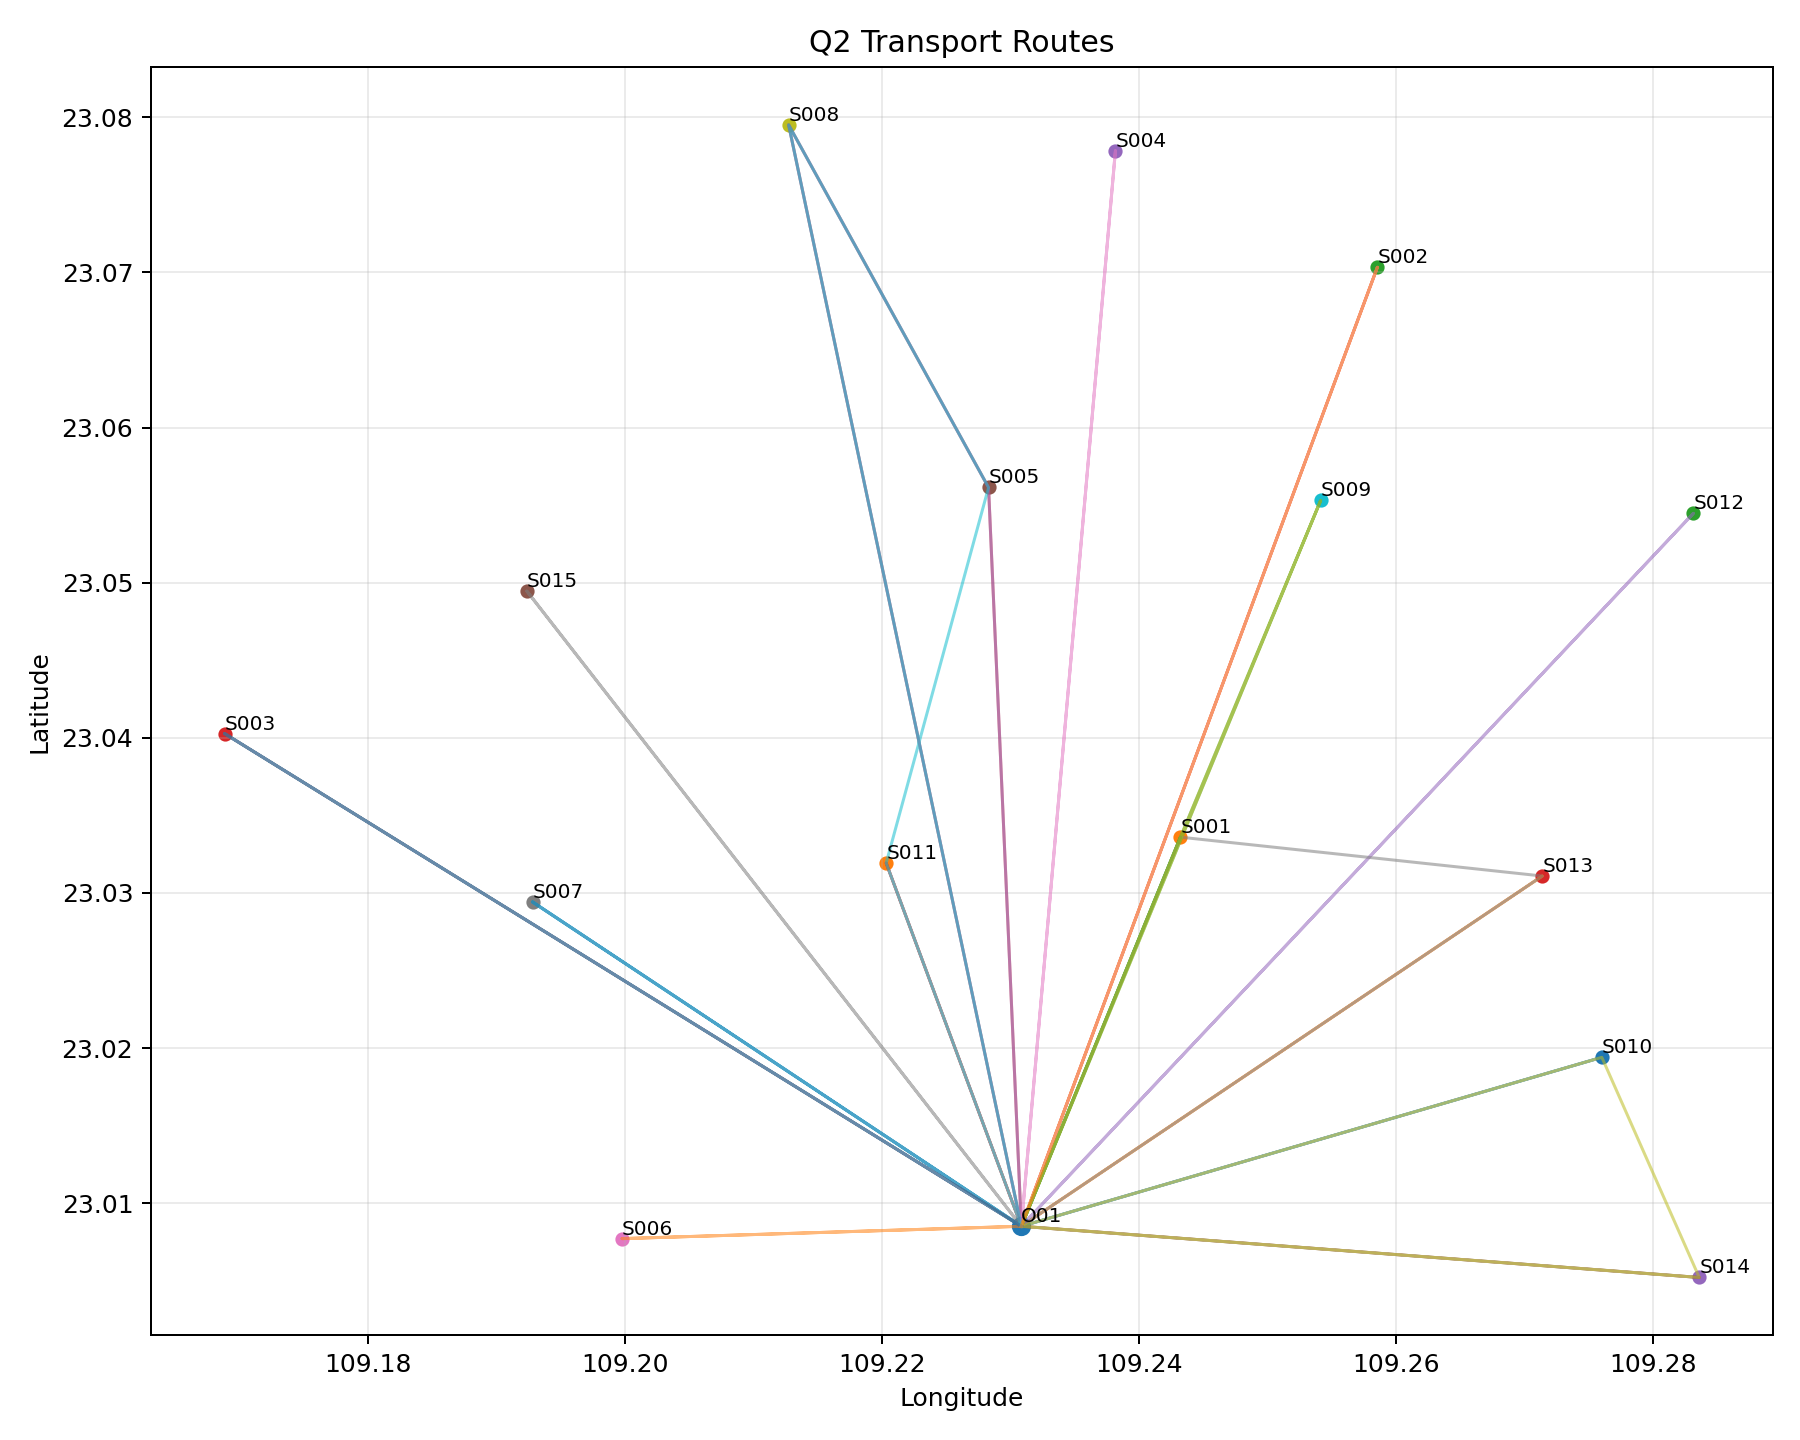
\includegraphics[width=0.90\linewidth]{../../code/2/output/fig1_routes.png}
	\caption{问题二运输架次路线分布}
	\label{fig:q2-routes}
\end{figure}
\FloatBarrier

图~\ref{fig:q2-routes} 给出了全部运输架次的服务区访问路线。
可以看出，部分空间邻近服务区被合并至同一架次，
从而减少 O01 与服务区之间的重复往返；
但受载质量、体积、地形爬升、能量及时间约束影响，
并非所有空间邻近节点均适合合并运输，
最终路线体现了空间距离与资源约束之间的综合权衡。

\subsubsection{无人机调度结果}

图~\ref{fig:q2-gantt} 给出了 8 架实体运输无人机的任务甘特图。
初始阶段，8 架无人机尽可能并行执行时限较紧的首批保障和医疗运输任务；
随着任务推进，各实体机根据返航时刻和同型满电电池的可用情况继续承担后续架次。
该调度方式能够充分利用多架无人机并行运输能力，
降低整体任务完成时间。

\begin{figure}[htbp]
	\centering
	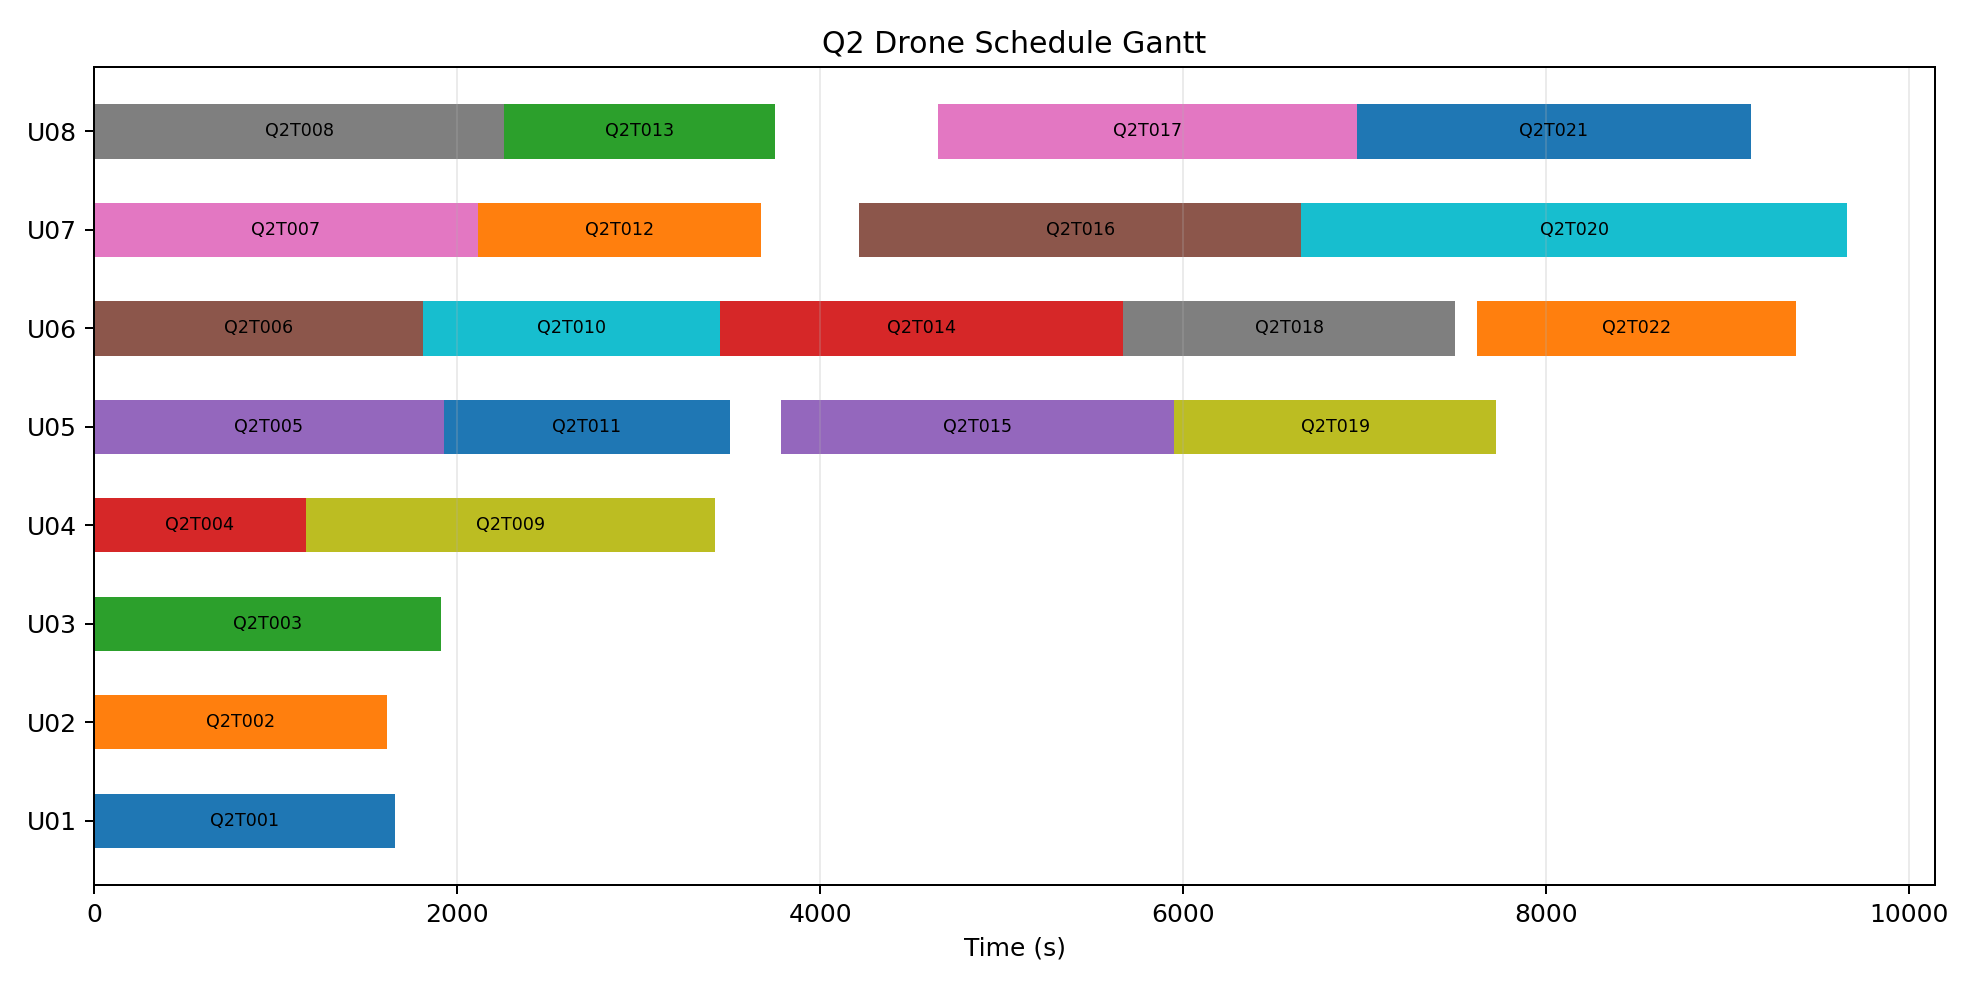
\includegraphics[width=0.95\linewidth]{../../code/2/output/fig2_gantt.png}
	\caption{问题二实体运输无人机调度甘特图}
	\label{fig:q2-gantt}
\end{figure}
\FloatBarrier

全部任务在 \QTwoMakespan~s 时完成并返回 O01。
根据最终调度结果，U01--U04 主要承担第一阶段的 A 型紧急运输任务，
B、C 型实体无人机则在后续阶段经过换电持续执行多轮运输，
体现了共享电池机制对提高实体无人机利用率的作用。

\subsubsection{逐箱配送及时性分析}

图~\ref{fig:q2-delivery} 将 80 个货箱按照期望送达时间排序，
比较实际交付完成时刻、期望送达时刻以及硬截止时刻。
其中硬截止点对应医疗物资和首批保障货箱。

\begin{figure}[htbp]
	\centering
	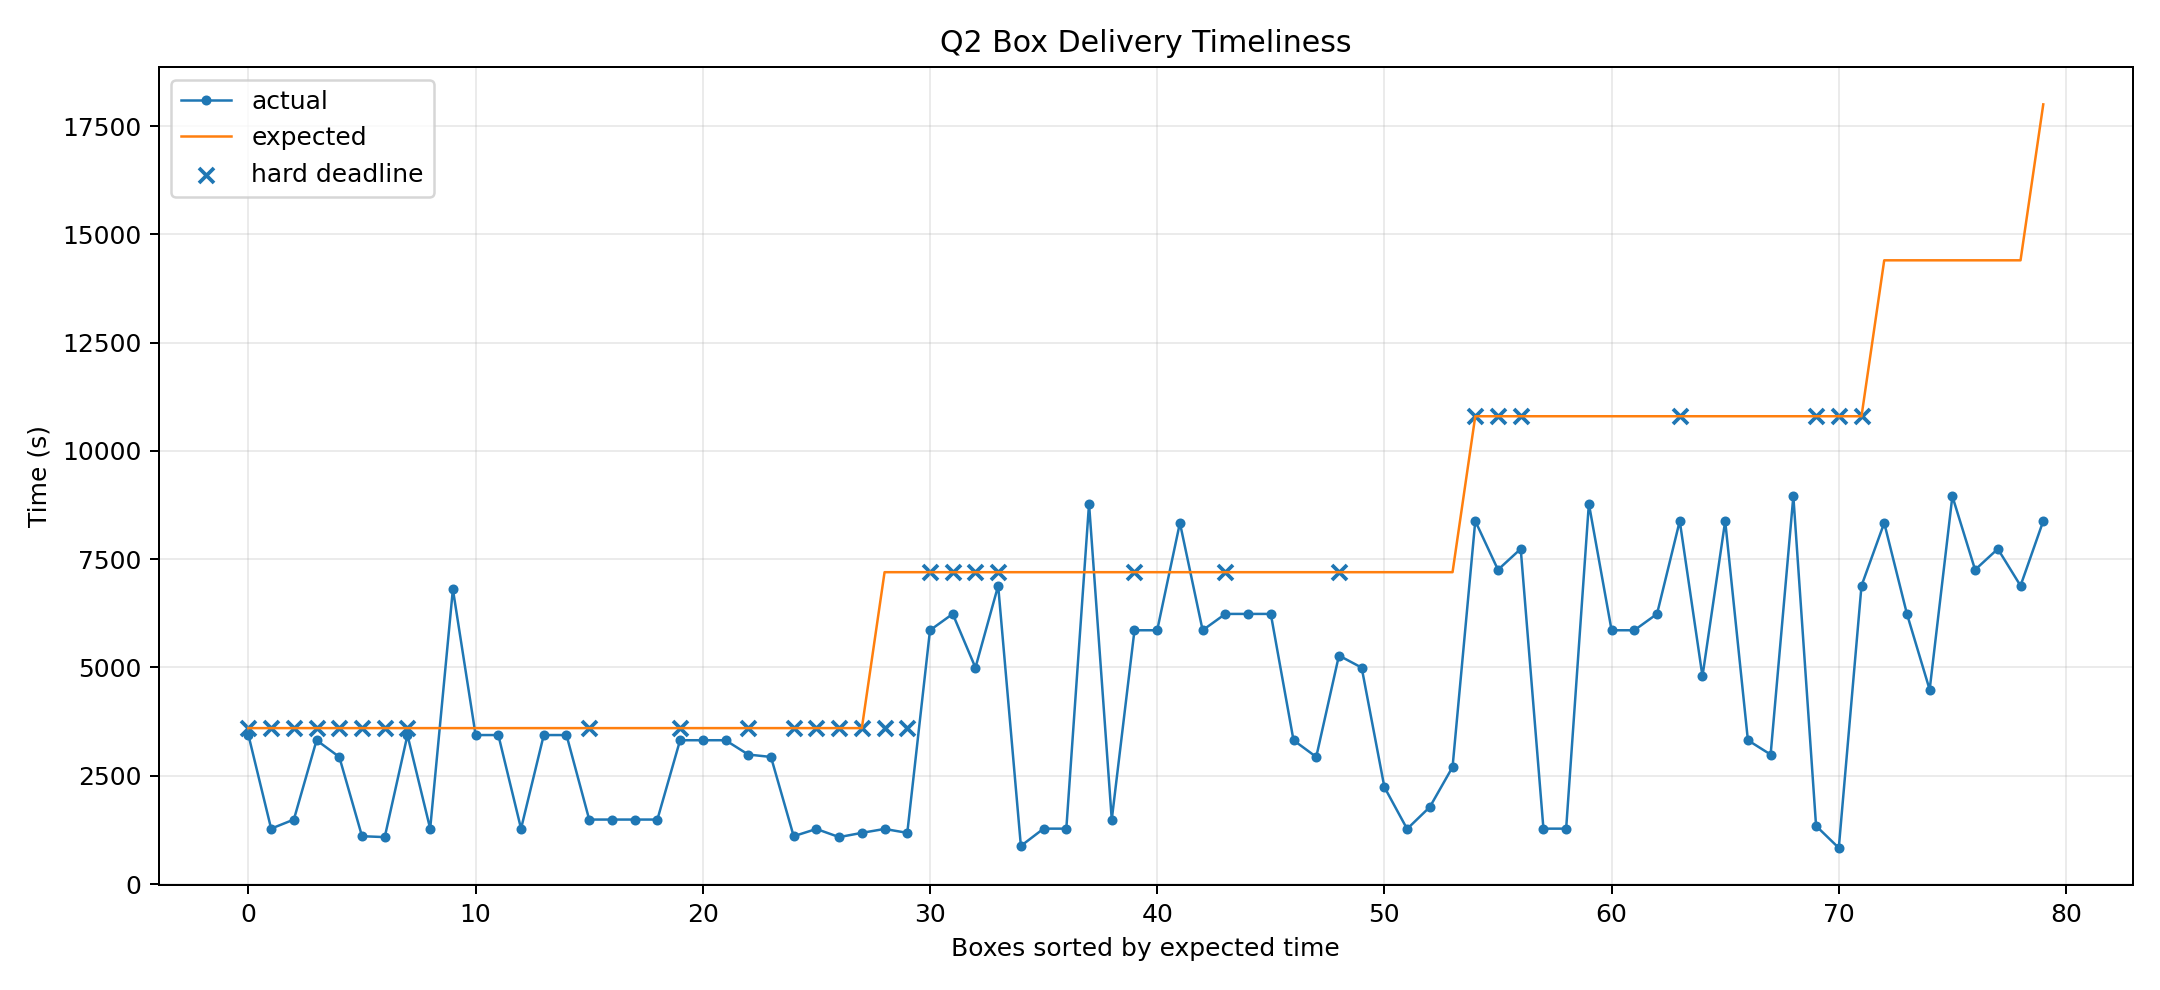
\includegraphics[width=0.95\linewidth]{../../code/2/output/fig3_delivery.png}
	\caption{问题二逐箱实际送达时刻与配送时限对比}
	\label{fig:q2-delivery}
\end{figure}
\FloatBarrier

计算结果表明，31 个具有硬时限要求的货箱全部按时完成交付，
硬时限违反数为 \QTwoHardViolation。
最终仅有 \QTwoSoftLateNum 个普通货箱超过其期望送达时间，
而普通物资的期望时间作为软约束计入加权迟到指标，
因此算法允许在必要时通过少量普通物资延迟，
换取整体架次数、能耗及关键救援物资及时性的改善。
这种处理能够体现灾后运输中
``首先保障医疗与首批应急物资，再兼顾一般物资整体效率''
的优先原则。

\subsubsection{共享电池周转分析}

图~\ref{fig:q2-battery} 给出了共享电池在任务执行与充电过程中的占用情况。
实心区间表示电池随无人机执行运输任务，
其后的空心区间表示该电池返航后恢复至 100\% SOC 所需的充电阶段。

\begin{figure}[htbp]
	\centering
	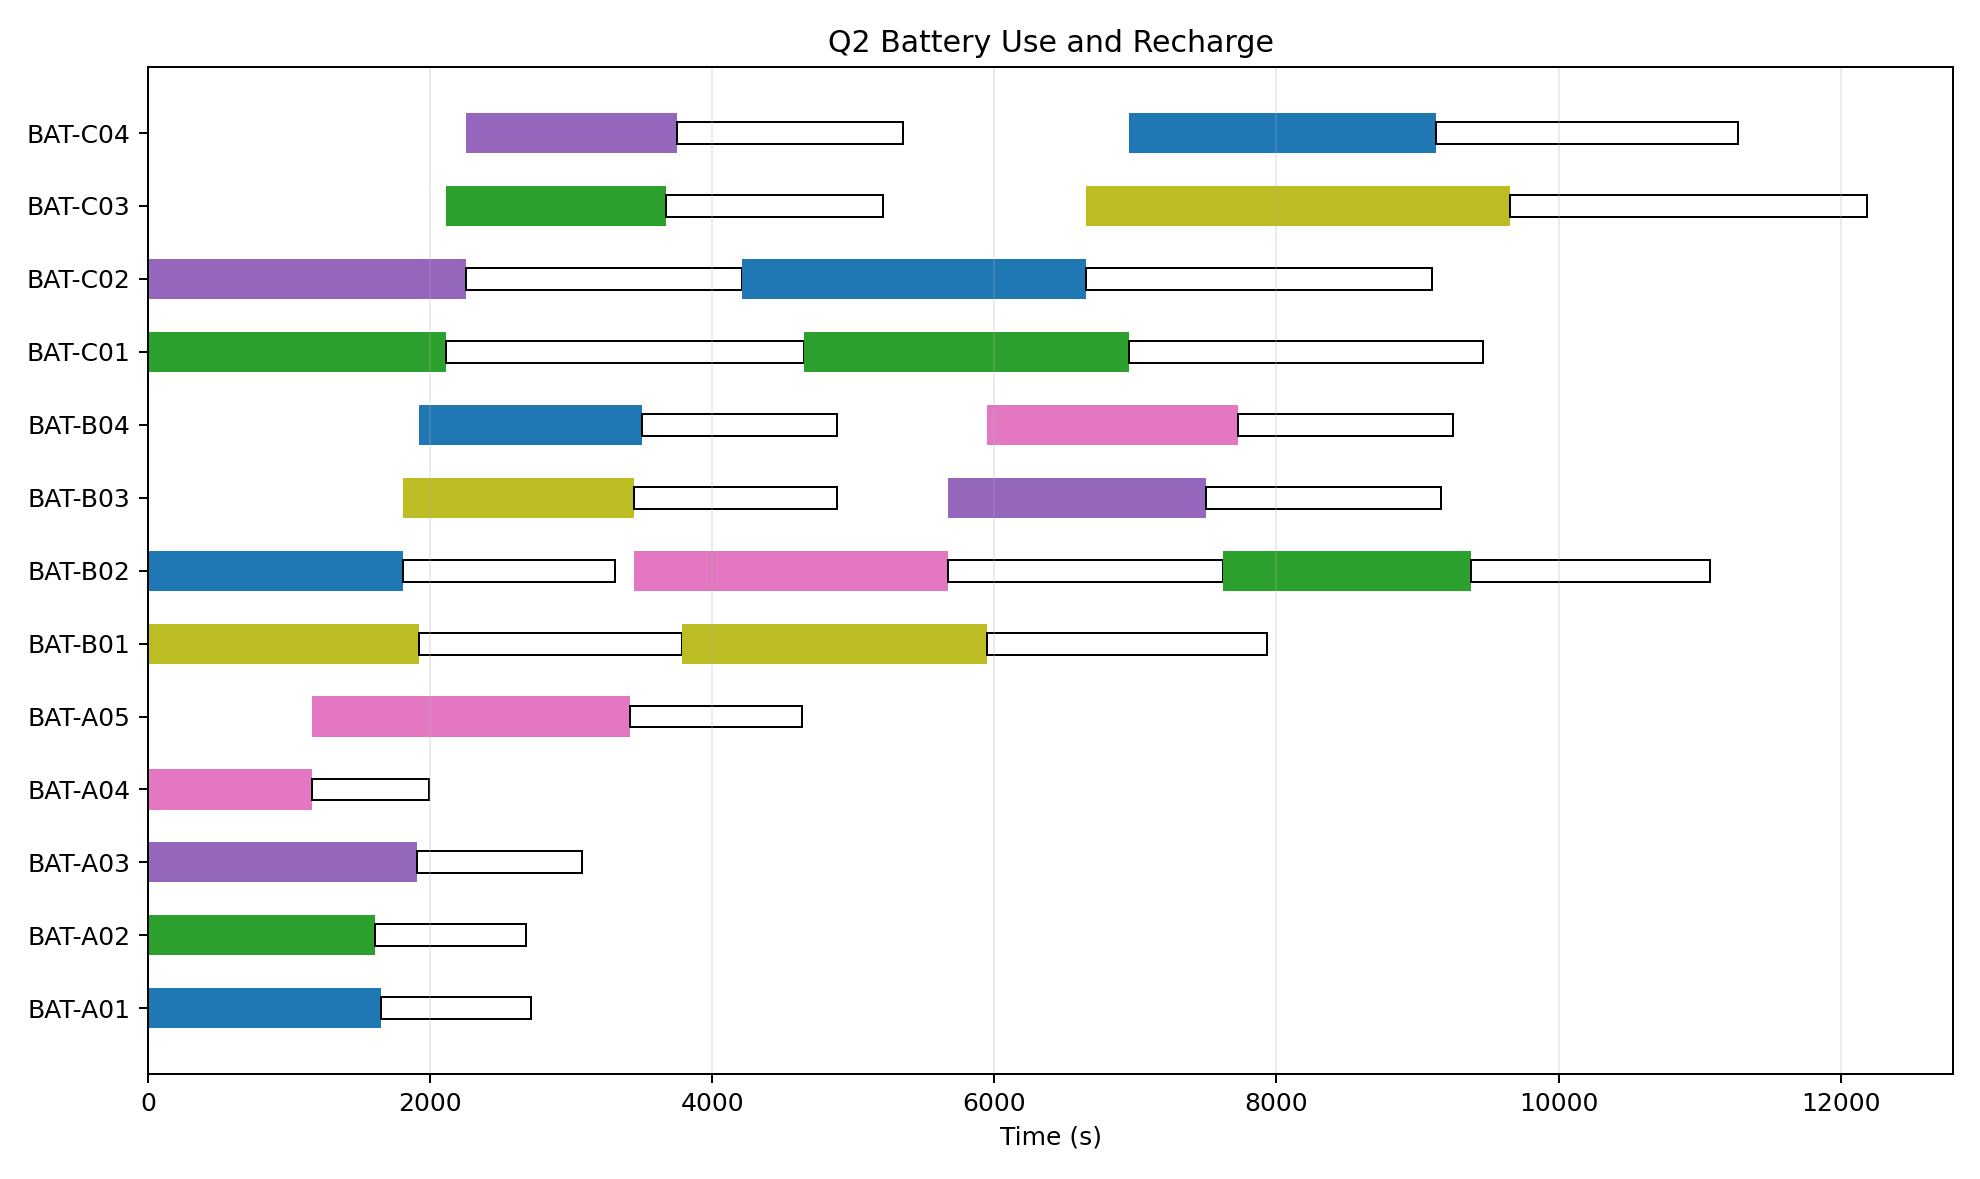
\includegraphics[width=0.95\linewidth]{../../code/2/output/fig4_battery.png}
	\caption{问题二共享电池使用与充电周转时序}
	\label{fig:q2-battery}
\end{figure}
\FloatBarrier

由调度结果可知，同一块共享电池的任务占用区间和充电区间均不存在重叠，
且再次投入任务前均已完成充电。
所有运输架次返航 SOC 均高于规定的安全下限，
其中最低返航 SOC 约为 \QTwoMinSOC，
说明最终方案在充分利用电池能量的同时仍满足返航安全余量约束。
由于实体无人机与电池采用独立资源池管理，
无人机返航后可以更换其他已充满的同型电池继续执行任务，
从而避免因单块电池充电造成整架无人机长时间闲置。

\subsubsection{ALNS 收敛性分析}

为考察启发式搜索过程，
记录迭代过程中历史最优归一化目标函数值，
结果如图~\ref{fig:q2-alns} 所示。

\begin{figure}[htbp]
	\centering
	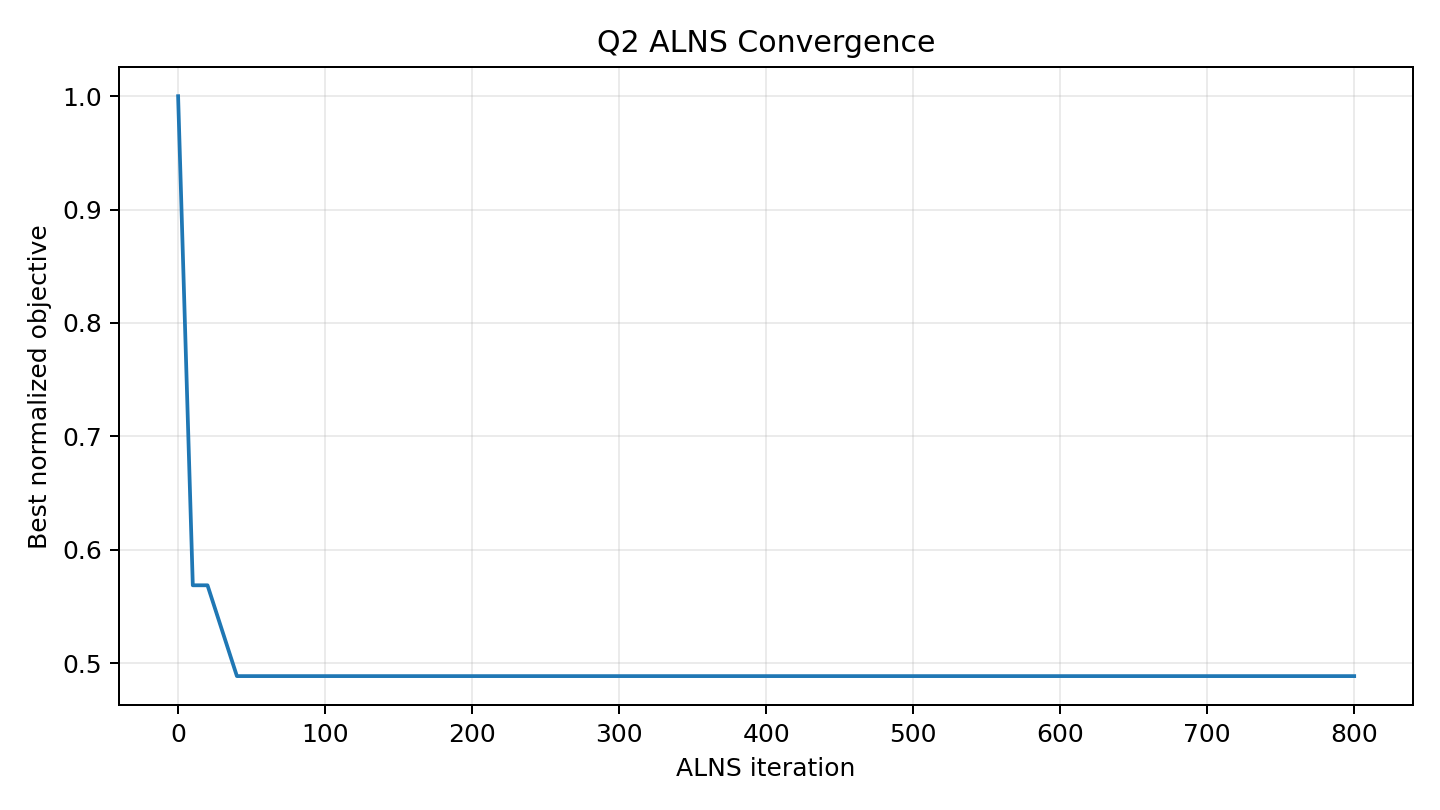
\includegraphics[width=0.78\linewidth]{../../code/2/output/fig5_alns.png}
	\caption{问题二 ALNS 迭代收敛曲线}
	\label{fig:q2-alns}
\end{figure}
\FloatBarrier

可以看出，算法在初始阶段通过货箱重新组合和路线合并迅速改善目标函数，
随后进入较缓慢的局部搜索阶段。
模拟退火接受机制使搜索过程中允许暂时接受部分较差方案，
从而为跳出局部最优提供可能；
随着温度下降，搜索逐渐集中于当前优质解邻域。
在 \QTwoIter 次迭代后，综合目标保持稳定，
说明当前参数设置下算法具有较好的收敛性。

\subsection{方案可行性检验}

为避免启发式算法得到数值较优但实际不可执行的方案，
程序在最终结果输出前设置独立的 Solution Validator，
对货箱、架次、实体无人机和共享电池进行完整审计。

首先，对全部 80 个货箱编号进行集合校验，
要求每个货箱有且仅有一个所属架次，
不存在遗漏配送、重复配送及目的服务区错误。
其次，对每一架次重新计算起飞载质量、装载体积、逐航段剩余载荷、
运输能耗和返航 SOC，
保证容量及返航安全余量均满足要求。
再次，根据逐箱交付时刻检查医疗物资及首批保障货箱的硬时限，
最终硬时限违反数为 \QTwoHardViolation。
最后，按照实体无人机编号和共享电池编号分别检查资源占用区间，
保证同一无人机不存在任务时间重叠，
同一电池不存在``执行任务--充电--再次执行''过程上的时间冲突。

经上述检验，最终方案满足
\[
\boxed{
	\text{货箱唯一交付}
	+
	\text{容量可行}
	+
	\text{能源可行}
	+
	\text{硬时限可行}
	+
	\text{无人机资源可行}
	+
	\text{共享电池资源可行}
}.
\]

因此，所得方案可以作为问题二的可执行运输调度方案。
需要说明的是，ALNS 属于启发式优化方法，
本文结果为当前搜索参数和随机种子下得到的较优可行解，
并不宣称其为严格意义上的全局最优解。

\subsection{结果文件与程序输出}

为保证论文结果与提交文件完全一致，
程序不再人工二次整理调度数据，
而是直接根据最终 Decoded Solution 自动生成结果文件。
其中，\texttt{Q2\_运输架次} 给出架次编号、无人机编号、
机型编号、电池编号、开始时刻、访问服务区顺序、
返回 O01 时刻和架次能耗；
\texttt{Q2\_逐箱交付} 给出 80 个货箱对应的架次编号、
服务区编号及实际交付完成时刻。

除正式结果模板外，
程序同时输出
\texttt{Q2\_详细结果.xlsx}、
\texttt{arc\_library.csv}、
架次与逐箱交付 CSV 文件，
以及路线图、无人机甘特图、逐箱及时性图、
共享电池周转图和 ALNS 收敛曲线，
从而保证建模过程、数值结果与最终提交文件之间具有一致的数据来源和可复现性。

% ============================================================
% 问题三：通信约束下的运输与中继联合调度方案
% 可直接替换模板中“问题三的模型建立与求解”部分
% ============================================================

% ---------- 问题三最终结果宏 ----------
% 若后续正式运行 q3_solver_joint_v2_1.py 后结果变化，只需修改本段宏
\newcommand{\QThreeSeed}{20260924}
\newcommand{\QThreeTransportIter}{0}
\newcommand{\QThreeJointIter}{20}

\newcommand{\QThreeBaseLate}{1131.054}
\newcommand{\QThreeBaseMakespan}{26461.112}
\newcommand{\QThreeBaseMakespanHour}{7.350}
\newcommand{\QThreeBaseEnergy}{90.744}
\newcommand{\QThreeBaseTrips}{38}

\newcommand{\QThreeLate}{752.950}
\newcommand{\QThreeMakespan}{26243.895}
\newcommand{\QThreeMakespanHour}{7.290}
\newcommand{\QThreeTransportEnergy}{83.015}
\newcommand{\QThreeRelayEnergy}{7.060}
\newcommand{\QThreeEnergy}{90.075}
\newcommand{\QThreeTransportTrips}{25}
\newcommand{\QThreeRelayTrips}{13}
\newcommand{\QThreeTrips}{38}
\newcommand{\QThreeHardViolation}{0}
\newcommand{\QThreeCommOutage}{0}
\newcommand{\QThreeScore}{0.846041}

\newcommand{\QThreeLateImprove}{33.43\%}
\newcommand{\QThreeMakespanImprove}{0.82\%}
\newcommand{\QThreeEnergyImprove}{0.74\%}
\newcommand{\QThreeScoreImprove}{15.40\%}

\section{问题三：通信约束下的运输与中继联合调度}
\label{sec:q3}

\subsection{问题分析与总体思路}

问题三在问题二异构运输无人机多点多架次调度的基础上，进一步要求运输无人机在
爬升、巡航、下降及物资投送全过程保持通信。
当运输无人机与固定网关 G01 的直连链路不可用时，
必须由空中中继无人机建立
“运输无人机--中继无人机--G01”两段链路，
并同时考虑中继悬停位置、悬停海拔、服务时段、中继实体机及能源组件周转。
因此，问题三实质上是一个同时包含
\textbf{运输路线、运输时序、通信覆盖、中继部署和双层能源资源调度}
的时空耦合优化问题。

无人机作为空中通信节点具有部署灵活、视距链路概率高等特点，
适用于地面通信基础设施受损后的临时覆盖与中继保障\cite{q3-zeng2016}；
同时，中继无人机三维位置会显著影响覆盖范围与持续服务能力，
因此悬停位置与高度不能脱离通信需求独立设置\cite{q3-mozaffari2016}。

若简单采用“先完成运输优化，再为每个运输架次配置中继”的顺序方法，
容易出现多个运输架次在不同空间盲区同时需要中继，
从而超过题目仅有的两架中继无人机容量。
为体现运输与通信的真正协同，本文构建独立的问题三求解器，
重新从原始附件读取运输、DEM、中继和通信数据，
在保持问题二统一飞行与能耗口径的同时，
将运输方案与通信保障共同纳入联合搜索。
整体求解流程为
\[
\boxed{
	\begin{aligned}
		&\text{原始数据读取与运输航段预计算}
		\rightarrow \text{运输可行方案构造} \\
		&\rightarrow \text{连续飞行轨迹离散化}
		\rightarrow \text{固定网关直连判定}
		\rightarrow \text{通信缺口聚类} \\
		&\rightarrow \text{中继候选点搜索与双中继覆盖}
		\rightarrow \text{中继资源解码} \\
		&\rightarrow \text{通信冲突反馈错峰}
		\rightarrow \text{通信感知 Joint-ALNS} \\
		&\rightarrow \text{联合方案审计与结果输出}.
\end{aligned}}
\]

其中，问题二中使用的运输 Route Evaluator、资源解码、载荷相关能耗和共享电池周转思想
在问题三程序中独立实现，不直接调用问题二求解器或其输出文件。
这样既保证两个问题的公共物理规则一致，又允许问题三根据通信约束重新调整货箱分配和运输时序。

\subsection{运输轨迹的时空展开}

设运输架次集合为 $\mathcal{R}^{T}$。
运输架次 $r\in\mathcal{R}^{T}$ 的服务区访问序列为
\[
O01\rightarrow i_{r1}\rightarrow i_{r2}
\rightarrow\cdots\rightarrow i_{rK_r}\rightarrow O01.
\]
运输部分的容量、逐段剩余载荷、飞行时间、载荷相关能耗、返航 SOC、
硬时限和共享电池周转均沿用问题二的计算口径。
多架次无人机配送与能源约束具有典型车辆路径与资源复用特征，
相关建模思想可参见 Dorling 等关于多架次无人机配送路径与能耗约束的研究\cite{q3-dorling2017}。

为了进行通信判定，需要将每一运输架次进一步展开为随时间变化的三维轨迹。
设运输无人机在时刻 $t$ 的位置为
\begin{equation}
	\mathbf{p}_r(t)
	=\left(\lambda_r(t),\varphi_r(t),H_r(t)\right),
	\label{eq:q3-trajectory}
\end{equation}
其中 $\lambda_r(t)$、$\varphi_r(t)$ 和 $H_r(t)$ 分别为经度、纬度和海拔。
对任一节点间航段，按照题目给定的“爬升--巡航--下降”三阶段规则进行线性时间插值；
服务区投送阶段则保持在服务区作业高度。

程序在通信规划阶段采用
\begin{equation}
	\Delta t=30\ \mathrm{s}
	\label{eq:q3-sample-step}
\end{equation}
的时间步长对完整飞行轨迹进行离散化，
并保留各飞行阶段端点附近的采样点。
因此，题目中的连续通信约束在数值实现中转化为对全部轨迹采样点的逐点可用性约束。

\subsection{通信链路模型}

\subsubsection{地形视距判定}

固定网关 G01 位于 O01，
其通信端点海拔由 O01 地面高程与网关天线离地高度共同确定。
对任意两个通信端点 $a,b$，
设三维位置分别为
\[
\mathbf{p}_a=(\lambda_a,\varphi_a,H_a),\qquad
\mathbf{p}_b=(\lambda_b,\varphi_b,H_b).
\]

沿两端点水平投影连线提取经过的 DEM 像元。
若某一中间 DEM 像元对应地面高程不低于两通信端点视线连线在该位置的高度，
则认为发生地形遮挡。
定义遮挡变量
\begin{equation}
	\chi_{ab}=
	\begin{cases}
		1,&\text{端点 }a,b\text{ 之间存在地形遮挡},\\
		0,&\text{否则}.
	\end{cases}
	\label{eq:q3-block}
\end{equation}

这种处理直接使用 30 m DEM 对山体遮挡进行判定，
从而避免仅依据二维距离估计山区通信覆盖范围。

\subsubsection{自由空间损耗与双向链路预算}

自由空间基本传播损耗按照 ITU-R P.525 建议书计算\cite{q3-itu525}。
设载波频率为 $f$ MHz，两通信端点三维距离为 $d_{ab}$ km，则
\begin{equation}
	L_{ab}^{\mathrm{FS}}
	=32.44+20\log_{10}f+20\log_{10}d_{ab}.
	\label{eq:q3-fspl}
\end{equation}

考虑地形遮挡附加损耗 $L^{\mathrm{obs}}$ 后，
总传播损耗定义为
\begin{equation}
	L_{ab}
	=L_{ab}^{\mathrm{FS}}
	+\chi_{ab}L^{\mathrm{obs}}.
	\label{eq:q3-total-loss}
\end{equation}

设接收灵敏度为 $P^{\mathrm{sens}}$，衰落裕量为 $M^{\mathrm{fade}}$，
则有效接收门限为
\begin{equation}
	P^{\mathrm{req}}
	=P^{\mathrm{sens}}+M^{\mathrm{fade}}.
	\label{eq:q3-receive-threshold}
\end{equation}

对于通信方向 $a\rightarrow b$，
最大允许总传播损耗为
\begin{equation}
	L_{a\rightarrow b}^{\max}
	=P_a^{t}+G_a^{t}+G_b^{r}
	-L^{\mathrm{sys}}-P^{\mathrm{req}},
	\label{eq:q3-oneway-budget}
\end{equation}
其中 $P_a^t$ 为发射功率，$G_a^t$、$G_b^r$ 分别为发射与接收天线增益，
$L^{\mathrm{sys}}$ 为系统损耗。
由于运输控制和状态回传均需可靠通信，
端点 $a,b$ 的双向链路预算取两个方向中的较小值：
\begin{equation}
	L_{ab}^{\max}
	=\min\left\{
	L_{a\rightarrow b}^{\max},
	L_{b\rightarrow a}^{\max}
	\right\}.
	\label{eq:q3-bidirectional-budget}
\end{equation}

因此，单链路可用变量定义为
\begin{equation}
	A_{ab}(t)
	=\mathbf{1}\left\{
	L_{ab}(t)\le L_{ab}^{\max}
	\right\}.
	\label{eq:q3-link-available}
\end{equation}

\subsubsection{运输无人机通信状态}

记运输架次 $r$ 与固定网关 G01 的链路状态为
$A_{rG}(t)$，
与中继架次 $q$ 的接入链路状态为 $A_{rq}(t)$，
中继架次 $q$ 与 G01 的回传链路状态为 $A_{qG}(t)$。
若 $z_{rq}(t)=1$ 表示时刻 $t$ 由中继架次 $q$ 为运输架次 $r$ 提供保障，
则有效通信状态为
\begin{equation}
	C_r(t)
	=A_{rG}(t)
	\vee
	\left[
	\bigvee_{q\in\mathcal{R}^{R}}
	z_{rq}(t)A_{rq}(t)A_{qG}(t)
	\right].
	\label{eq:q3-communication-state}
\end{equation}

所有运输轨迹采样点均要求满足
\begin{equation}
	C_r(t)=1,
	\qquad r\in\mathcal{R}^{T},
	\label{eq:q3-continuous-constraint}
\end{equation}
且同一运输无人机在同一时刻最多由一架中继无人机提供通信保障：
\begin{equation}
	\sum_{q\in\mathcal{R}^{R}}z_{rq}(t)\le 1.
	\label{eq:q3-one-relay}
\end{equation}

若 $A_{rG}(t)=0$，则将该时刻记为中继通信需求点。
程序将时间上相邻的需求点聚合成通信缺口，
从而避免为每一个离散采样点单独产生中继任务。

\subsection{中继悬停位置与中继架次模型}

\subsubsection{中继候选位置生成}

设中继候选悬停点为
\[
c=(\lambda_c,\varphi_c,H_c),
\]
其水平位置必须位于 DEM 覆盖区域内，
悬停离地高度满足
\begin{equation}
	0<H_c-H_c^{\mathrm{DEM}}
	\le H_R^{\max}.
	\label{eq:q3-relay-height}
\end{equation}

为避免在全部 DEM 像元上进行穷举，
本文采用“通信缺口驱动的局部候选搜索”。
首先围绕失联轨迹采样点在 DEM 网格上构造候选位置，
并取若干代表性离地高度
\[
H^{\mathrm{AGL}}\in\{150,225,300\}\ \mathrm{m}.
\]
候选点首先必须满足中继--G01 回传链路可用。
随后检查其对当前通信缺口内运输轨迹采样点的覆盖情况。

对于同一时间簇，程序优先寻找一个可完整覆盖全部需求点的悬停位置；
若单点不能满足，则利用位集覆盖搜索寻找两个候选点的组合。
若粗网格下仍存在少量未覆盖采样点，
则仅在未覆盖轨迹附近加密 DEM 候选点，
避免全局细网格搜索造成过大的计算开销。
由于题目仅配置两架中继无人机，
若某一并发时间簇仍需要超过两个相互不兼容的空间中继簇，
则将该冲突反馈至运输调度层，通过错峰调整运输架次开始时刻。

\subsubsection{中继飞行与服务时间}

中继架次 $q$ 的完整任务为
\[
O01\rightarrow c_q
\rightarrow\text{悬停通信服务}
\rightarrow O01.
\]
中继从 O01 到悬停点的计划巡航海拔同样取沿线最高 DEM 高程以上 50 m。
设中继固定准备时间为 $t_R^{\mathrm{pre}}$，
飞抵悬停点所需时间为 $t_q^{\mathrm{out}}$，
建链时间为 $t_R^{\mathrm{link}}$，
通信需求开始时刻为 $s_q^{\mathrm{serv}}$，
则必须满足
\begin{equation}
	s_q^{R}
	+t_R^{\mathrm{pre}}
	+t_q^{\mathrm{out}}
	+t_R^{\mathrm{link}}
	\le s_q^{\mathrm{serv}},
	\label{eq:q3-relay-ready}
\end{equation}
其中 $s_q^R$ 为中继架次开始时刻。
若提前到达，中继在悬停点等待至服务开始，该等待时间同样计入悬停与通信能耗。

\subsubsection{中继能耗与返航安全约束}

设中继巡航功率、悬停功率和通信附加功率分别为
$P_R^{c}$、$P_R^{h}$ 与 $P_R^{\mathrm{com}}$，
水平单程巡航时间为 $t_q^{c}$，
往返累计爬升高度为 $h_q^{+}$，
计划起飞总质量为 $M_R$，爬升效率为 $\eta_R^{\uparrow}$。
则中继往返飞行能耗为
\begin{equation}
	E_q^{\mathrm{fly}}
	=
	2P_R^c\frac{t_q^{c}}{3600}
	+
	\frac{M_Rgh_q^{+}}
	{3.6\times10^6\eta_R^{\uparrow}}.
	\label{eq:q3-relay-flight-energy}
\end{equation}

若服务持续时间为 $T_q^{\mathrm{serv}}$，
则建链和通信服务阶段能耗为
\begin{equation}
	E_q^{\mathrm{hov}}
	=
	\left(P_R^h+P_R^{\mathrm{com}}\right)
	\frac{t_R^{\mathrm{link}}+T_q^{\mathrm{serv}}}{3600}.
	\label{eq:q3-relay-hover-energy}
\end{equation}

因此中继架次总能耗为
\begin{equation}
	E_q^R
	=E_q^{\mathrm{fly}}+E_q^{\mathrm{hov}}.
	\label{eq:q3-relay-total-energy}
\end{equation}

若中继能源组件可用能量为 $E_R^{\mathrm{bat}}$，
返航安全余量比例为 $\rho_R$，则必须满足
\begin{equation}
	E_q^R\le
	(1-\rho_R)E_R^{\mathrm{bat}},
	\label{eq:q3-relay-reserve}
\end{equation}
相应返航 SOC 为
\begin{equation}
	SOC_q^{R}
	=1-\frac{E_q^R}{E_R^{\mathrm{bat}}}
	\ge \rho_R.
	\label{eq:q3-relay-soc}
\end{equation}

中继能源组件的充电仍采用附件规定的两阶段等效充电模型。
同一中继无人机的两个任务区间不得重叠，
同一能源组件在“执行任务--充电--再次执行”的整个过程中不得发生资源冲突。

\subsection{通信冲突反馈与联合调度解码}

仅根据空间覆盖生成中继任务仍可能产生两类冲突：
一是同一时刻出现三个及以上相互不兼容的通信空间簇；
二是虽然空间上只需两架中继，但上一中继架次尚未返航或完成周转，
使 R01、R02 在新的通信需求开始前均不可用。

为此，程序设置外层通信联合修复机制。
当出现通信覆盖冲突时，从当前并发运输架次中优先选择时间裕量较大的架次进行错峰；
当出现中继实体机或能源组件冲突时，
根据最早可用资源时刻计算所需延迟量，并反馈至运输架次最早开始时间。
随后重新运行运输资源解码器，重新生成运输轨迹并再次规划中继。
该过程迭代至同时满足
\[
\boxed{
	\text{运输资源可行}
	+\text{硬时限可行}
	+\text{通信覆盖可行}
	+\text{中继资源可行}
}.
\]

上述反馈机制可以快速获得一份完整可行的运输--中继联合基线，
但由于其主要通过保守错峰消除冲突，
可能导致普通物资明显延迟。
因此，在可行基线之上进一步执行通信感知 Joint-ALNS。

\subsection{多目标联合优化模型}

设货箱 $b$ 的应急优先系数为 $p_b$，
实际交付完成时刻为 $T_b^{\mathrm{del}}$，
期望送达时刻为 $D_b^E$。
沿用问题二的加权迟到指标
\begin{equation}
	J_L
	=\sum_{b\in\mathcal B}
	p_b
	\frac{\max\{0,T_b^{\mathrm{del}}-D_b^E\}}
	{D_b^E}.
	\label{eq:q3-lateness}
\end{equation}

问题三的联合任务完成时间必须同时考虑运输无人机和中继无人机：
\begin{equation}
	C_{\max}^{J}
	=
	\max\left\{
	\max_{r\in\mathcal R^T}F_r^T,
	\max_{q\in\mathcal R^R}F_q^R
	\right\}.
	\label{eq:q3-joint-makespan}
\end{equation}

运输与中继总能耗为
\begin{equation}
	E_{\mathrm{tot}}^{J}
	=\sum_{r\in\mathcal R^T}E_r^T
	+\sum_{q\in\mathcal R^R}E_q^R,
	\label{eq:q3-joint-energy}
\end{equation}
总架次数为
\begin{equation}
	N_{\mathrm{tot}}^{J}
	=|\mathcal R^T|+|\mathcal R^R|.
	\label{eq:q3-joint-trips}
\end{equation}

以通信联合修复得到的完整可行基线为归一化基准，
记四项指标基准值为
$J_L^0$、$C_0^J$、$E_0^J$ 和 $N_0^J$，
构造联合目标函数
\begin{equation}
	F_J
	=0.45\frac{J_L}{J_L^0}
	+0.25\frac{C_{\max}^{J}}{C_0^J}
	+0.20\frac{E_{\mathrm{tot}}^{J}}{E_0^J}
	+0.10\frac{N_{\mathrm{tot}}^{J}}{N_0^J}.
	\label{eq:q3-joint-objective}
\end{equation}

其中配送及时性仍赋予最高权重，
联合完工时间次之，总能耗与两类无人机使用架次作为资源效率指标。
医疗物资及首批保障货箱硬时限、运输容量、运输返航安全余量、连续通信、中继返航安全余量及资源冲突
均作为硬约束，不参与加权折中。

\subsection{通信感知 Joint-ALNS 求解算法}

ALNS 通过多种 Destroy/Repair 算子在大邻域内重构路线，
并依据历史表现自适应调整算子使用频率，
适合求解具有容量、时间窗和多资源约束的复杂路径问题\cite{q3-ropke2006}。
针对问题三中“运输路径变化会同时改变通信需求”的特点，
本文在传统 ALNS 基础上设计通信感知结构算子，
将当前联合状态记为
\[
\mathcal S
=(\mathcal R^T,\boldsymbol{\ell},\Pi_T,\Pi_R),
\]
其中 $\mathcal R^T$ 为运输路线集合，
$\boldsymbol{\ell}$ 为各路线最早释放时刻，
$\Pi_T$ 与 $\Pi_R$ 分别表示运输和中继资源调度结果。

\subsubsection{Communication-conflict destroy}

普通随机移除无法针对中继瓶颈进行搜索。
因此，本文首先计算每一运输路线的中继占用时长
\begin{equation}
	B_r
	=\Delta t
	\sum_{k}
	\mathbf 1\{A_{rG}(t_k)=0\},
	\label{eq:q3-relay-burden}
\end{equation}
并结合该路线货箱迟到贡献构造通信冲突评分
\begin{equation}
	S_r^{\mathrm{des}}
	=4L_r
	+0.8\frac{B_r}{600}
	+0.25\frac{s_r}{7200},
	\label{eq:q3-destroy-score}
\end{equation}
其中 $L_r$ 为路线内普通货箱迟到贡献，$s_r$ 为路线实际开始时刻。
算法优先从高分路线中移除 1--2 个不存在硬时限的普通货箱，
并要求被破坏路线至少保留一个货箱，
以避免一次结构变化过大造成大面积不可行。

该算子的本质是优先寻找
“\textbf{送得晚且占用中继时间长}”的路线，
使后续 Repair 有机会把其中普通货箱迁移到更早、通信几何更友好的运输架次。

\subsubsection{Relay-aware repair}

对于被移除货箱 $b$，
依次尝试插入其它物理可行运输路线。
若目标路线已访问货箱所属服务区，则优先直接并入已有停靠点；
否则才尝试增加新的服务区停靠点。
这是因为同服务区回插基本不改变原运输路径的空间几何，
通常不会额外产生新的通信盲区。

对候选插入位置，构造通信感知代理代价
\begin{equation}
	\begin{aligned}
		C_{b\rightarrow r}^{\mathrm{rep}}
		={}&\Delta C_{r}^{\mathrm{proxy}}
		+0.75D_{br}
		+2.2L_{br}^{\mathrm{est}} \\
		&+0.15\frac{B_r}{600}
		+P_{br}^{\mathrm{dir}}
		-3I_{br}^{\mathrm{same}}
		-0.00018\Delta T_b
		+2.5I_{br}^{\mathrm{return}},
	\end{aligned}
	\label{eq:q3-repair-score}
\end{equation}
其中 $D_{br}$ 为新增服务区与路线已有停靠点之间的空间距离代理量，
$L_{br}^{\mathrm{est}}$ 为估计迟到代价，
$P_{br}^{\mathrm{dir}}$ 用于惩罚新增且固定网关直连条件较差的服务区，
$I_{br}^{\mathrm{same}}$ 表示目标路线是否已访问同一服务区，
$\Delta T_b$ 表示相对当前方案的提前送达量，
$I_{br}^{\mathrm{return}}$ 用于惩罚货箱重新回到原路线。
若候选插入违反硬时限，则直接排除。

对每个待修复货箱，采用 Regret 思想比较最优和次优插入位置，
优先处理“若错过当前最佳位置则后续代价显著上升”的货箱。
这样可以在改善及时性的同时尽量避免增加新的中继空间簇。

\subsubsection{时间协同邻域与接受准则}

除结构邻域外，Joint-ALNS 同时设置以下时间协同算子：

\begin{enumerate}[label=(\arabic*),leftmargin=3em]
	\item \textbf{advance-one}：尝试提前一个已被通信修复推迟的运输架次；
	\item \textbf{advance-pair}：同时提前两个运输架次，增强组合搜索能力；
	\item \textbf{reset-one}：取消一个路线的附加释放时间，重新交由资源解码器调度；
	\item \textbf{exchange-shift}：提前一个架次，同时把另一条时间裕量较大的路线适度后移，
	通过交换并发关系减轻中继资源冲突；
	\item \textbf{conflict-destroy-repair}：执行上述通信冲突 Destroy 与中继感知 Repair，直接改变货箱所属路线。
\end{enumerate}

每个候选解都必须重新运行运输资源解码、运输轨迹生成、固定网关通信判定、
中继候选搜索和中继资源解码。
只要出现硬时限违反、通信覆盖失败、中继实体机冲突或能源组件冲突，
候选解即判为不可行。

若候选联合目标优于当前解则直接接受；
对于一定程度的劣解，仍采用模拟退火概率
\begin{equation}
	P_{\mathrm{acc}}
	=\exp\left(-\frac{F_J^{\mathrm{new}}-F_J^{\mathrm{cur}}}{T_k}\right)
	\label{eq:q3-sa}
\end{equation}
决定是否接受，其中
\begin{equation}
	T_k
	=\max\left\{0.004,
	0.07\left(1-\frac{k}{K}\right)
	\right\}.
	\label{eq:q3-temperature}
\end{equation}
结构算子初始权重设为 3.2，
高于普通时间邻域，以保证有限迭代次数下能够充分搜索运输路线结构；
各算子权重根据接受及改进情况动态调整。

本文问题三程序随机种子取 \QThreeSeed，
正式计算中运输层先采用保守可行基线，
随后执行 \QThreeJointIter 次通信感知 Joint-ALNS。

\begin{table}[htbp]
	\centering
	\caption{问题三主要算法参数}
	\label{tab:q3-parameters}
	\begin{tabularx}{0.90\linewidth}{Y Y}
		\toprule
		参数 & 取值 \\
		\midrule
		通信规划时间步长 $\Delta t$ & 30 s \\
		中继候选离地高度 & 150、225、300 m \\
		单架次最大访问服务区数 & 4 \\
		运输层 ALNS 迭代次数 & \QThreeTransportIter \\
		Joint-ALNS 迭代次数 & \QThreeJointIter \\
		配送及时性权重 & 0.45 \\
		联合完工时间权重 & 0.25 \\
		运输与中继总能耗权重 & 0.20 \\
		运输与中继总架次数权重 & 0.10 \\
		Joint-ALNS 初始温度 & 0.07 \\
		Joint-ALNS 最低温度 & 0.004 \\
		随机种子 & \QThreeSeed \\
		\bottomrule
	\end{tabularx}
\end{table}
\FloatBarrier

\subsection{求解结果与分析}

\subsubsection{总体优化结果}

首先通过通信冲突反馈与中继资源解码得到完整可行基线。
该基线的加权迟到指标为 \QThreeBaseLate，
联合任务完成时间为 \QThreeBaseMakespan~s，
即约 \QThreeBaseMakespanHour~h，
运输与中继总能耗为 \QThreeBaseEnergy~kWh，
运输与中继总架次数为 \QThreeBaseTrips。

经过通信感知 Joint-ALNS 后，
最终加权迟到指标降至 \QThreeLate，
联合任务完成时间为 \QThreeMakespan~s，
即约 \QThreeMakespanHour~h；
其中运输总能耗为 \QThreeTransportEnergy~kWh，
中继总能耗为 \QThreeRelayEnergy~kWh，
合计 \QThreeEnergy~kWh。
最终共包含 \QThreeTransportTrips 个运输架次和 \QThreeRelayTrips 个中继架次，
总架次数为 \QThreeTrips，
硬时限违反数为 \QThreeHardViolation，
通信中断采样点数为 \QThreeCommOutage。

\begin{table}[htbp]
	\centering
	\caption{问题三通信联合修复基线与 Joint-ALNS 方案对比}
	\label{tab:q3-result-summary}
	\resizebox{\linewidth}{!}{
		\begin{tabular}{lccccc}
			\toprule
			方案 & 加权迟到指标 & 联合完成时间/s & 总能耗/kWh & 总架次数 & 通信中断采样点 \\
			\midrule
			通信联合修复基线
			& \QThreeBaseLate & \QThreeBaseMakespan & \QThreeBaseEnergy & \QThreeBaseTrips & 0 \\
			Joint-ALNS 方案
			& \QThreeLate & \QThreeMakespan & \QThreeEnergy & \QThreeTrips & \QThreeCommOutage \\
			\midrule
			改善幅度
			& \QThreeLateImprove & \QThreeMakespanImprove & \QThreeEnergyImprove & 0 & -- \\
			\bottomrule
	\end{tabular}}
\end{table}
\FloatBarrier

由表~\ref{tab:q3-result-summary} 可见，
Joint-ALNS 在保持运输架次和中继架次数不增加的条件下，
使加权迟到指标降低约 \QThreeLateImprove，
联合完工时间缩短约 \QThreeMakespanImprove，
总能耗下降约 \QThreeEnergyImprove。
归一化联合目标由 1.000000 降至 \QThreeScore，
总体下降约 \QThreeScoreImprove。

架次数没有继续下降并不意味着结构优化无效。
本题只有两架中继无人机，运输路线合并过度可能导致多个空间通信盲区在时间上同时出现，
反而使中继系统无法覆盖。
因此，最终算法主要通过
“\textbf{把晚期普通货箱迁移至已有同服务区的较早架次}”
改善配送及时性，
并在不增加通信空间复杂度的前提下降低后续中继负担。
这说明问题三的最优方向并非单纯追求更少运输架次，
而是需要在运输效率和通信可保障性之间进行协同权衡。

\subsubsection{运输路线与中继悬停位置}

图~\ref{fig:q3-routes-relay} 给出了最终运输路线与中继悬停位置。
图中调度中心、服务区、中继悬停点和中继部署航线分别采用不同标记，
便于观察运输路线与通信保障位置之间的空间关系。

\begin{figure}[htbp]
	\centering
	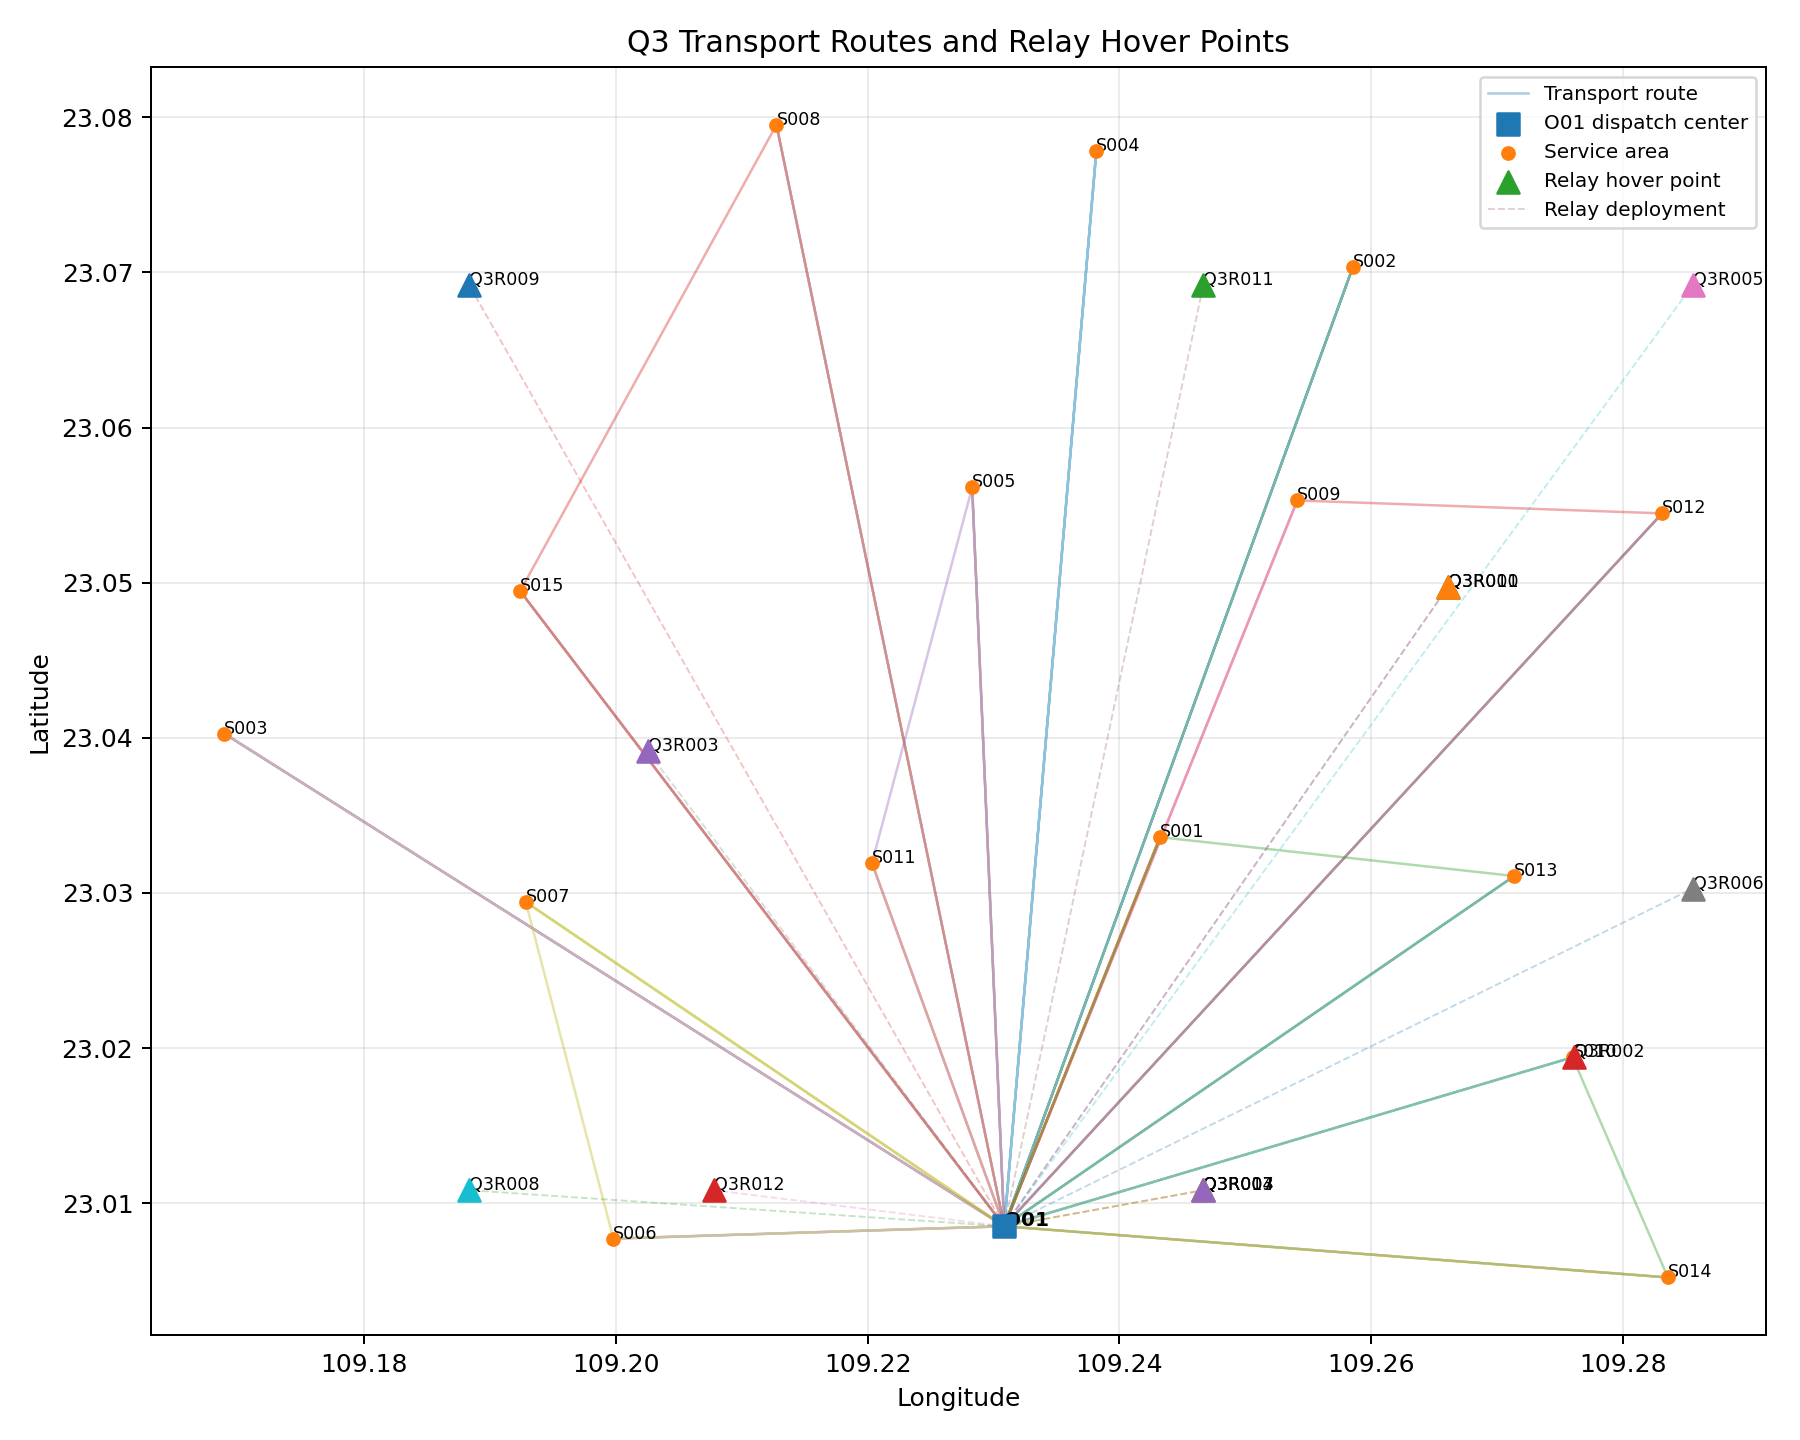
\includegraphics[width=0.95\linewidth]{../../code/3/output/fig_q3_1_routes_relay.png}
	\caption{问题三运输路线与中继悬停位置分布}
	\label{fig:q3-routes-relay}
\end{figure}
\FloatBarrier

可以看出，中继悬停点并未简单设置在服务区正上方，
而是由 DEM 地形、回传链路、运输轨迹及两架中继的联合覆盖需求共同决定。
部分悬停点可在同一服务时段覆盖多条运输轨迹，
从而避免为每个运输架次单独配置一架中继。

\subsubsection{运输--中继联合调度时序}

图~\ref{fig:q3-joint-gantt} 给出了运输无人机与中继无人机的联合调度甘特图。
运输任务与中继任务在同一时间轴上展示，
可直接观察通信需求出现前中继是否已经完成准备、飞抵和建链。

\begin{figure}[htbp]
	\centering
	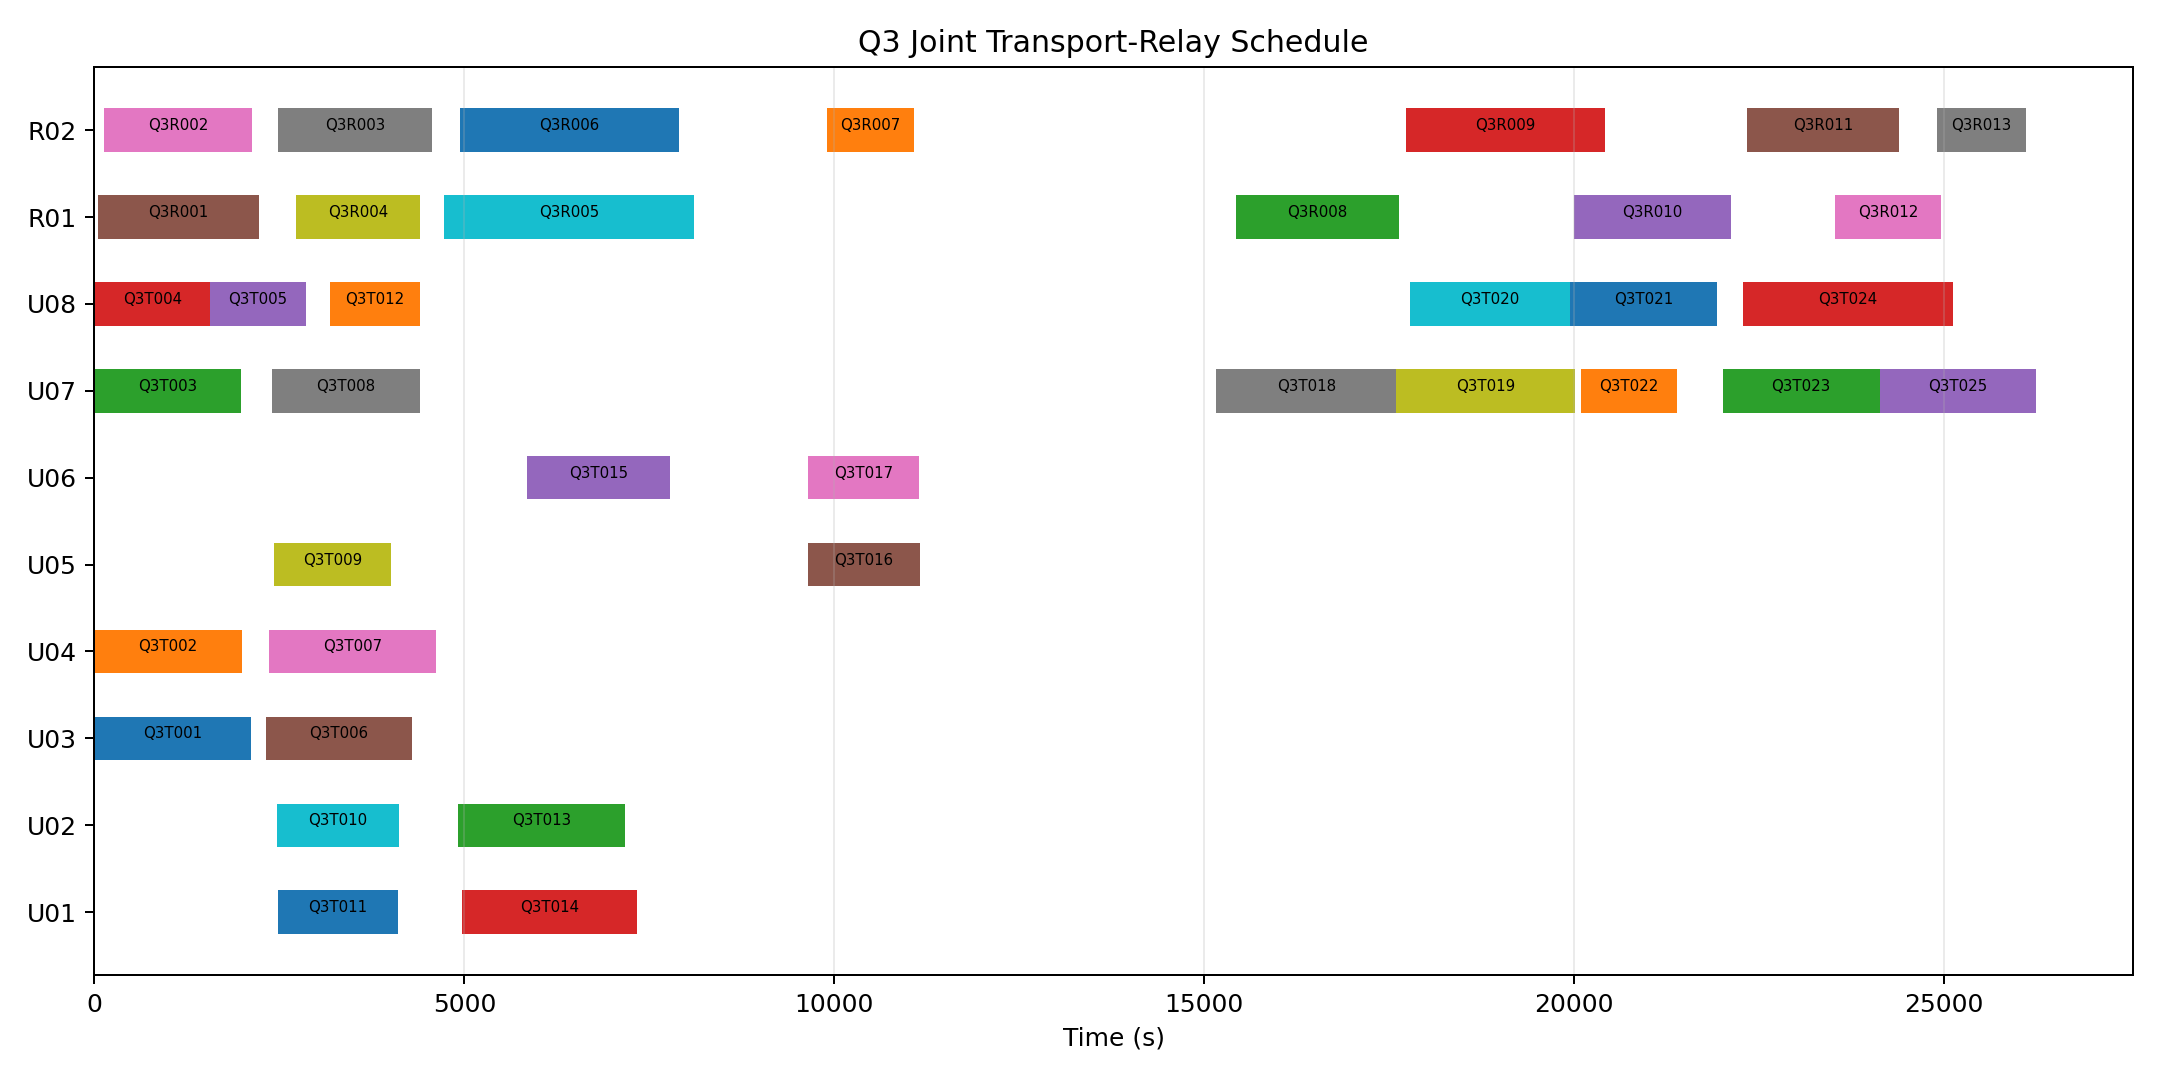
\includegraphics[width=0.96\linewidth]{../../code/3/output/fig_q3_2_joint_gantt.png}
	\caption{问题三运输无人机与中继无人机联合调度甘特图}
	\label{fig:q3-joint-gantt}
\end{figure}
\FloatBarrier

最终使用 \QThreeRelayTrips 个中继架次。
中继并非全程伴随运输无人机飞行，
而仅在固定网关直连不可用的时间段进入服务状态，
因此减少了无效悬停时间和额外通信能耗。

\subsubsection{连续通信保障状态}

图~\ref{fig:q3-comm-timeline} 按运输架次给出了固定网关直连与中继保障的时间分段。
当固定网关链路可用时优先采用直连；
进入山体遮挡或链路预算不足区间后切换至中继，
离开通信盲区后重新恢复直连。

\begin{figure}[htbp]
	\centering
	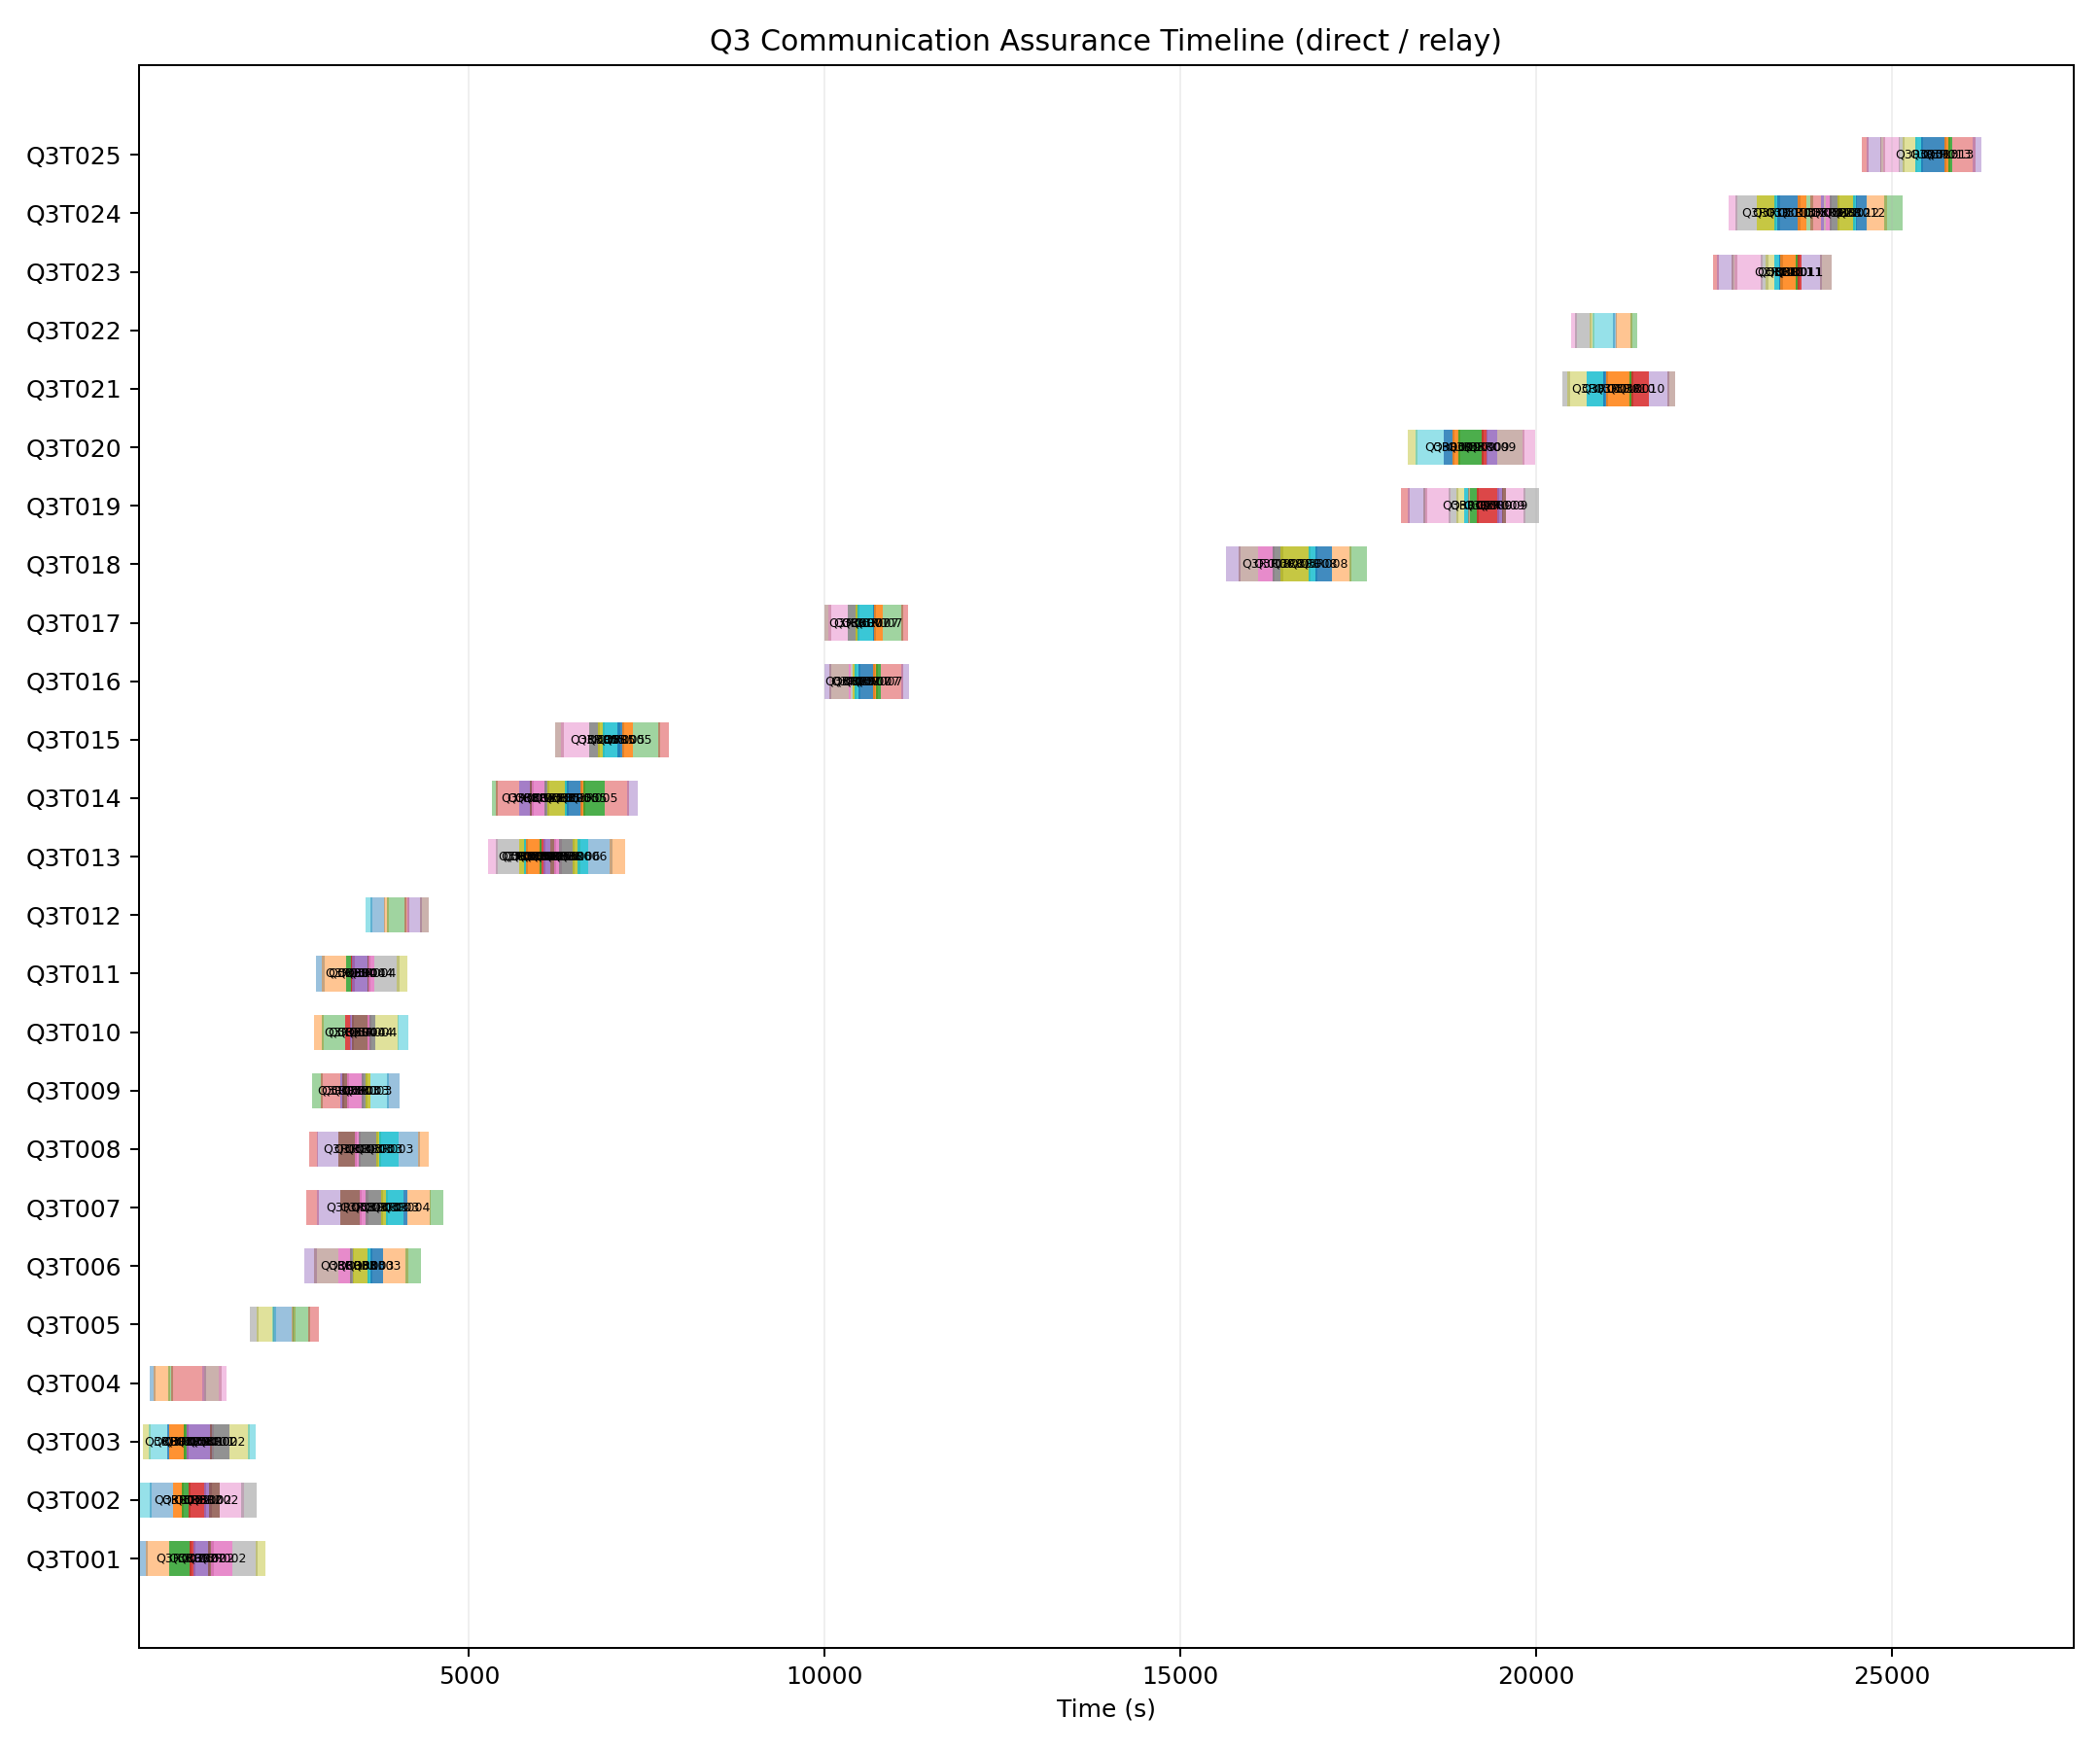
\includegraphics[width=0.97\linewidth]{../../code/3/output/fig_q3_3_comm_timeline.png}
	\caption{问题三各运输架次通信保障状态时间轴}
	\label{fig:q3-comm-timeline}
\end{figure}
\FloatBarrier

按照程序的 30 s 通信规划离散口径，
最终所有运输轨迹采样点均满足式~\eqref{eq:q3-communication-state}，
通信中断采样点数为 \QThreeCommOutage。
这表明固定网关直连与空中中继能够在整个运输任务过程中形成连续的数值覆盖链路。

\subsubsection{中继能耗与能源组件周转}

图~\ref{fig:q3-relay-energy} 给出了各中继架次能耗。
最终中继系统总能耗为 \QThreeRelayEnergy~kWh，
占运输与中继总能耗的比例较小，
说明按通信缺口部署中继比全程伴随式通信保障更加节能。

\begin{figure}[htbp]
	\centering
	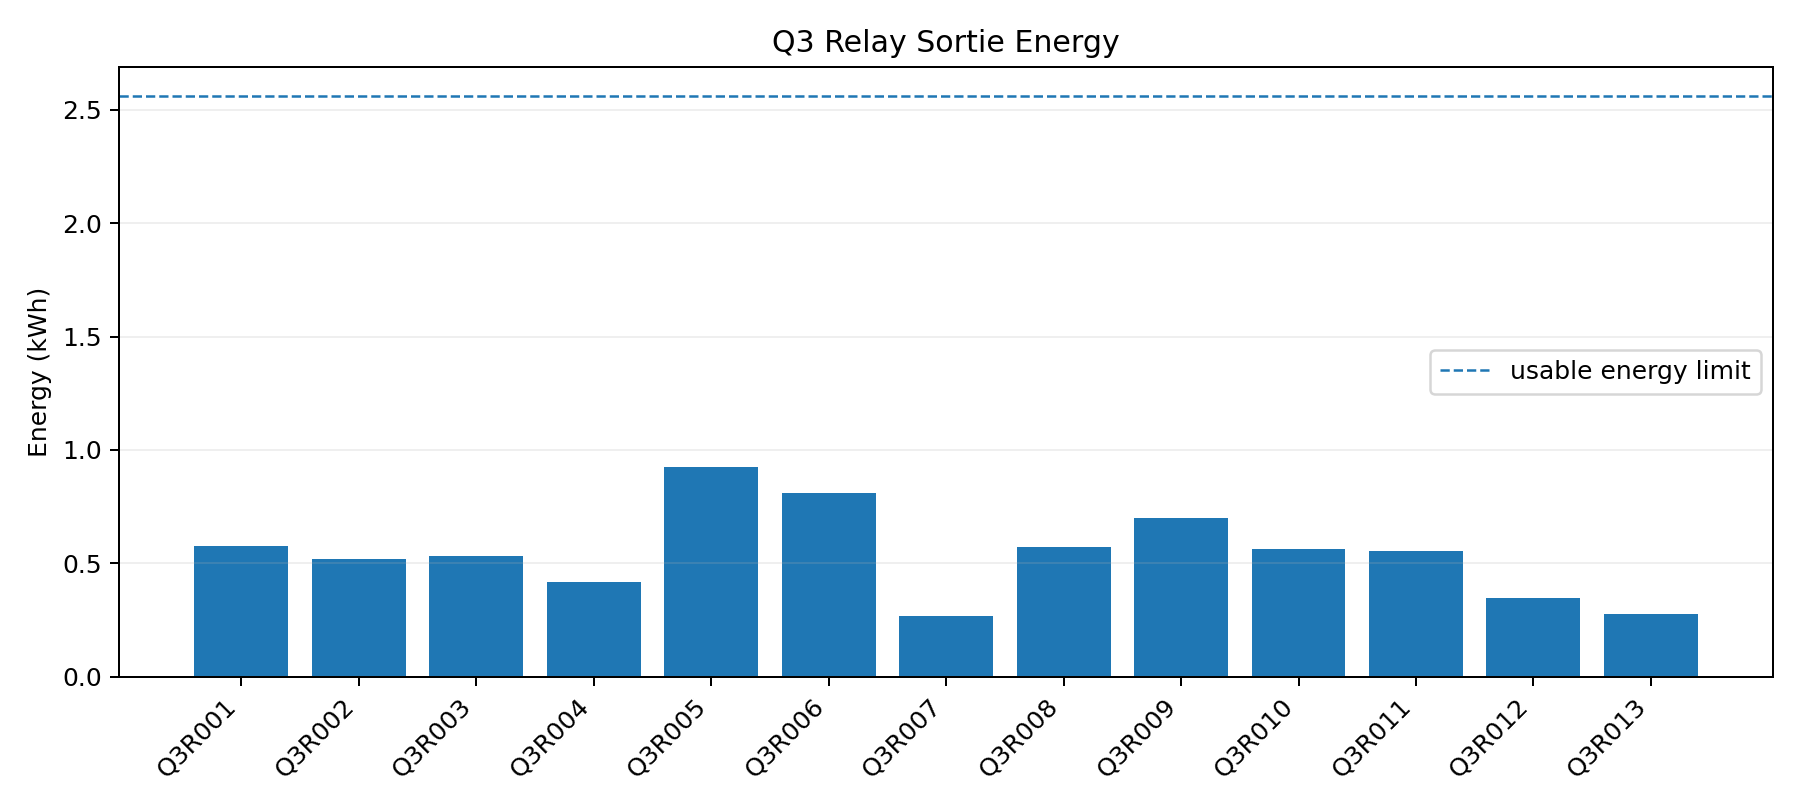
\includegraphics[width=0.90\linewidth]{../../code/3/output/fig_q3_4_relay_energy.png}
	\caption{问题三各中继架次能耗}
	\label{fig:q3-relay-energy}
\end{figure}
\FloatBarrier

所有中继架次均满足返航安全余量约束，
且 R01、R02 的任务占用时段不存在重叠；
六组能源组件按照“任务占用--返航--充电--再次可用”的顺序周转，
同一能源组件不存在并发占用。

\subsubsection{Joint-ALNS 收敛性分析}

图~\ref{fig:q3-joint-alns} 给出了通信感知 Joint-ALNS 的历史最优联合目标。
由于基线已经满足全部硬约束，初始归一化目标为 1。
结构算子开始起作用后，目标函数呈阶梯式下降，
最终稳定在 \QThreeScore。

\begin{figure}[htbp]
	\centering
	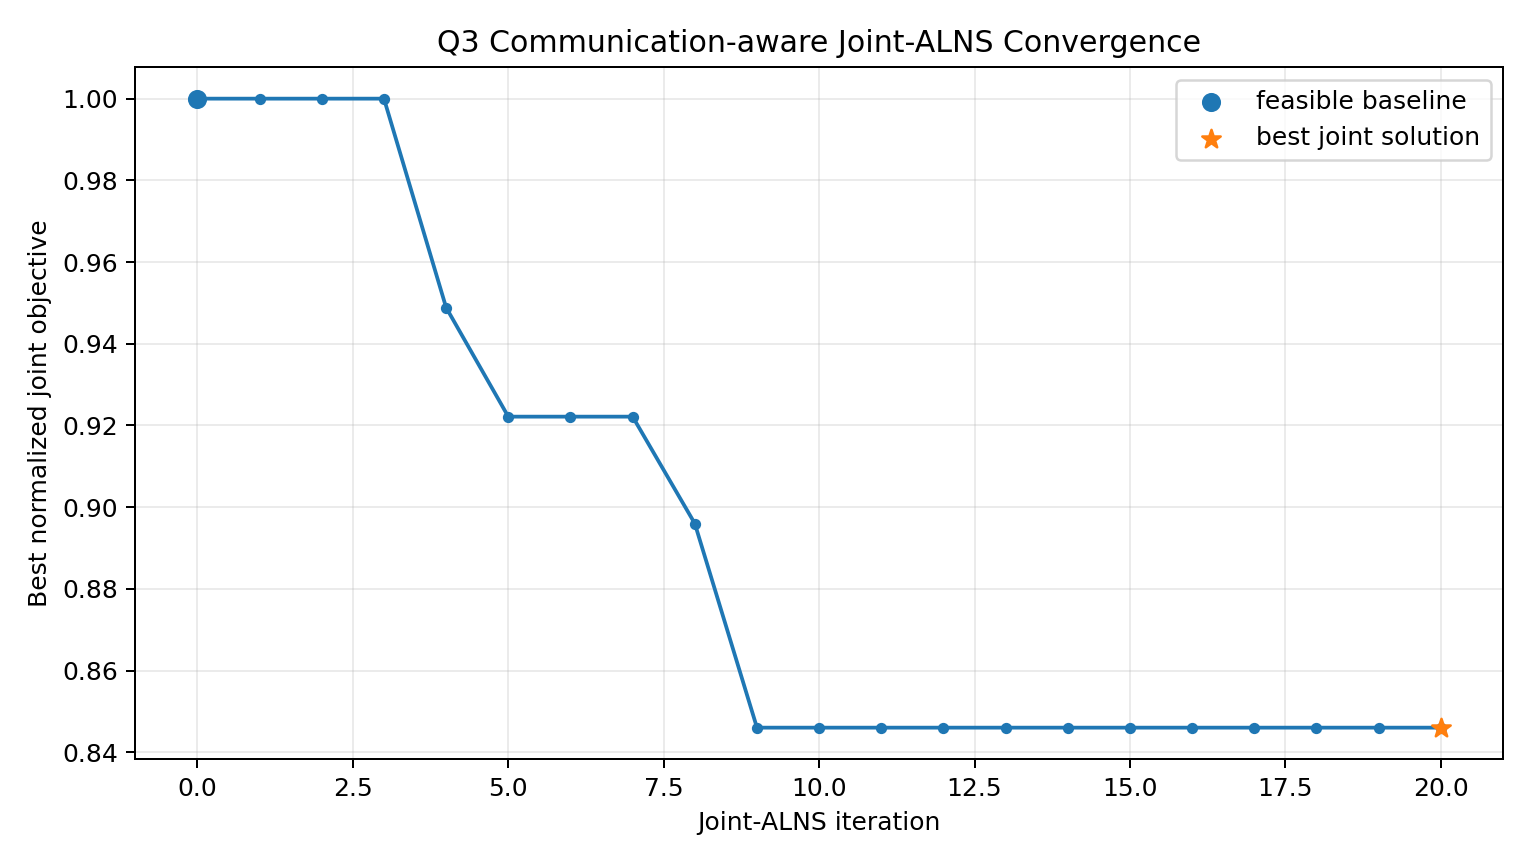
\includegraphics[width=0.82\linewidth]{../../code/3/output/fig_q3_7_joint_alns.png}
	\caption{问题三通信感知 Joint-ALNS 收敛曲线}
	\label{fig:q3-joint-alns}
\end{figure}
\FloatBarrier

搜索过程中，communication-conflict destroy 优先选取迟到贡献和中继占用均较大的路线，
relay-aware repair 则将部分普通货箱提前并入通信几何相容的早期路线。
因此，联合目标的主要改善来自配送及时性的显著提高，
同时联合完工时间和总能耗也得到小幅下降。

\subsection{方案可行性检验}

问题三比问题二多出通信链路、中继无人机和中继能源组件三类可行性条件。
为避免启发式算法产生“目标值较优但无法执行”的结果，
程序在候选状态评价和最终输出阶段均进行完整审计：

\begin{enumerate}[label=(\arabic*),leftmargin=3em]
	\item \textbf{货箱与运输路线：}
	80 个货箱均有且仅有一次交付，目的服务区正确；
	\item \textbf{运输容量与能源：}
	每个运输架次均满足载质量、体积和返航 SOC 安全余量；
	\item \textbf{配送时限：}
	医疗物资及首批保障货箱全部满足硬截止要求，
	最终硬时限违反数为 \QThreeHardViolation；
	\item \textbf{通信链路：}
	对所有运输轨迹通信采样点检查固定网关直连或中继两段链路，
	最终通信中断采样点数为 \QThreeCommOutage；
	\item \textbf{中继无人机资源：}
	同一中继无人机的架次占用时段不重叠，
	且每次均在通信需求开始前完成准备、飞抵和建链；
	\item \textbf{中继能源组件：}
	每次中继任务满足返航安全余量，
	同一能源组件的任务和充电时段不存在冲突，再次投入任务前完成充电。
\end{enumerate}

因此，最终方案满足
\[
\boxed{
	\begin{aligned}
		&\text{货箱唯一交付}
		+\text{运输容量可行}
		+\text{运输能源可行}\\
		&+\text{硬时限可行}
		+\text{通信保障可行}
		+\text{中继能源可行}\\
		&+\text{运输/中继实体资源可行}.
\end{aligned}}
\]

需要说明的是，本文采用的 Joint-ALNS 属于启发式联合优化方法，
所得结果是在当前候选点生成方式、时间离散精度、算法参数与随机种子下得到的较优可行解，
不宣称为严格意义上的全局最优解。
此外，连续通信在程序中采用 30 s 时间离散进行数值判定；
若需要进一步提高通信边界附近的验证精度，可在最终审计阶段缩小时间步长进行局部复核。

\subsection{结果文件与程序输出}

问题三程序为独立可运行文件
\texttt{q3\_solver\_joint\_v2\_1.py}，
直接读取原始节点、货箱、运输无人机、中继无人机、通信链路和 DEM 数据，
不依赖问题二求解器或问题二结果文件。

程序自动回填结果模板中的
\texttt{Q3\_中继架次} 和 \texttt{Q3\_通信保障} 两个工作表。
其中前者记录中继无人机编号、能源组件编号、开始时刻、悬停经纬度与海拔、
建链完成时刻、服务结束时刻、返航时刻及架次能耗；
后者按照通信阶段将每个运输架次的状态压缩为连续时间区间，
标记其采用“直连”或具体中继架次保障。

此外，程序输出
\texttt{Q3\_详细结果.xlsx}、
\texttt{Q3\_Joint\_ALNS日志.csv}、
中继架次与通信保障 CSV，
以及运输--中继空间分布图、联合甘特图、通信状态时间轴、
中继能耗图、通信方式占比图和 Joint-ALNS 收敛图，
从而保证论文中的主要结论与正式提交结果具有统一的数据来源和可复现性。


\section{模型评价与改进}
\subsection{优点与局限}
\Placeholder{优点对应已验证的效果，局限说明对结果的实际影响，不写空泛评价。}

\subsection{改进方向}
\Placeholder{提出具体改进方法、所需数据与验证方式，区分已完成的工作和未来计划。}

\section{结论}
\Placeholder{逐项回应赛题任务，概括最重要的量化结果、意义及成立条件，不引入正文未展示的新实验或新数字。引用网上资料时核实来源及访问日期\cite{web-placeholder}。}
